	\documentclass{article}
\usepackage[margin=1in]{geometry}
\title{COMP3811: Computer Graphics\\Coursework 2\\Interactive Animated Scenes with OpenGL}
\author{Joe Jeffcock\\sid: 201172812\\sc18j3j}

\usepackage{float}
\usepackage{tabularx}
\usepackage{graphicx}
\usepackage[justification=centering]{caption}
\graphicspath{{images/},{../src/textures/}}
\usepackage{hyperref}
\hypersetup{colorlinks=true}

\begin{document}
	\hypersetup{linkcolor=black}
	\maketitle
	\tableofcontents
	\hypersetup{linkcolor=blue, urlcolor=cyan}

	\clearpage
	\section{Introduction}
	Horror films from the mid-to-late 20th century have a unique atmosphere due in part to their use of shadows.
	The stark contrast between lit and unlit surfaces allowed for dramatic effects that involved the manipulation of
	light sources to generate interesting shadows.
	
	\bigskip
	
	Working with lighting in OpenGL, I was immediately inspired by Alfred Hitchcock's Psycho (1960) to create an
	atmospheric 3D scene with heavily contrasting shadows and moving light sources.
	
	\bigskip
	
	The scene would make use of OpenGL to present dramatic texturing and lighting of objects in the scene,
	and feature various animated instances of oscillation to create a visually interesting atmosphere. Complex geometry
	required would also present an opportunity to learn skills in 3D modelling software, a personal and
	professional goal of mine towards my interests in art and robotics.
	
	
	\subsection{Aims}
	\begin{itemize}
		\item Meet the requirements of each band of the project specification.
		\item Learn how to create convex objects from polygons using OpenGL and 3DS Max.
		\item Create a scene with the visual atmosphere of a 20th century horror film.
	\end{itemize}
	\subsection{Context}
	To better contextualise the report of this project, the final result of the visual scene
	is given by Figure \ref{final}. %TODO ref
	This representation will hopefully give motivation to some of the design choices that may not be easily
	conveyed by the drafts and graph plots created during the initial phases of development.
	
	\bigskip

	\begin{figure}[h]
		\centering	
		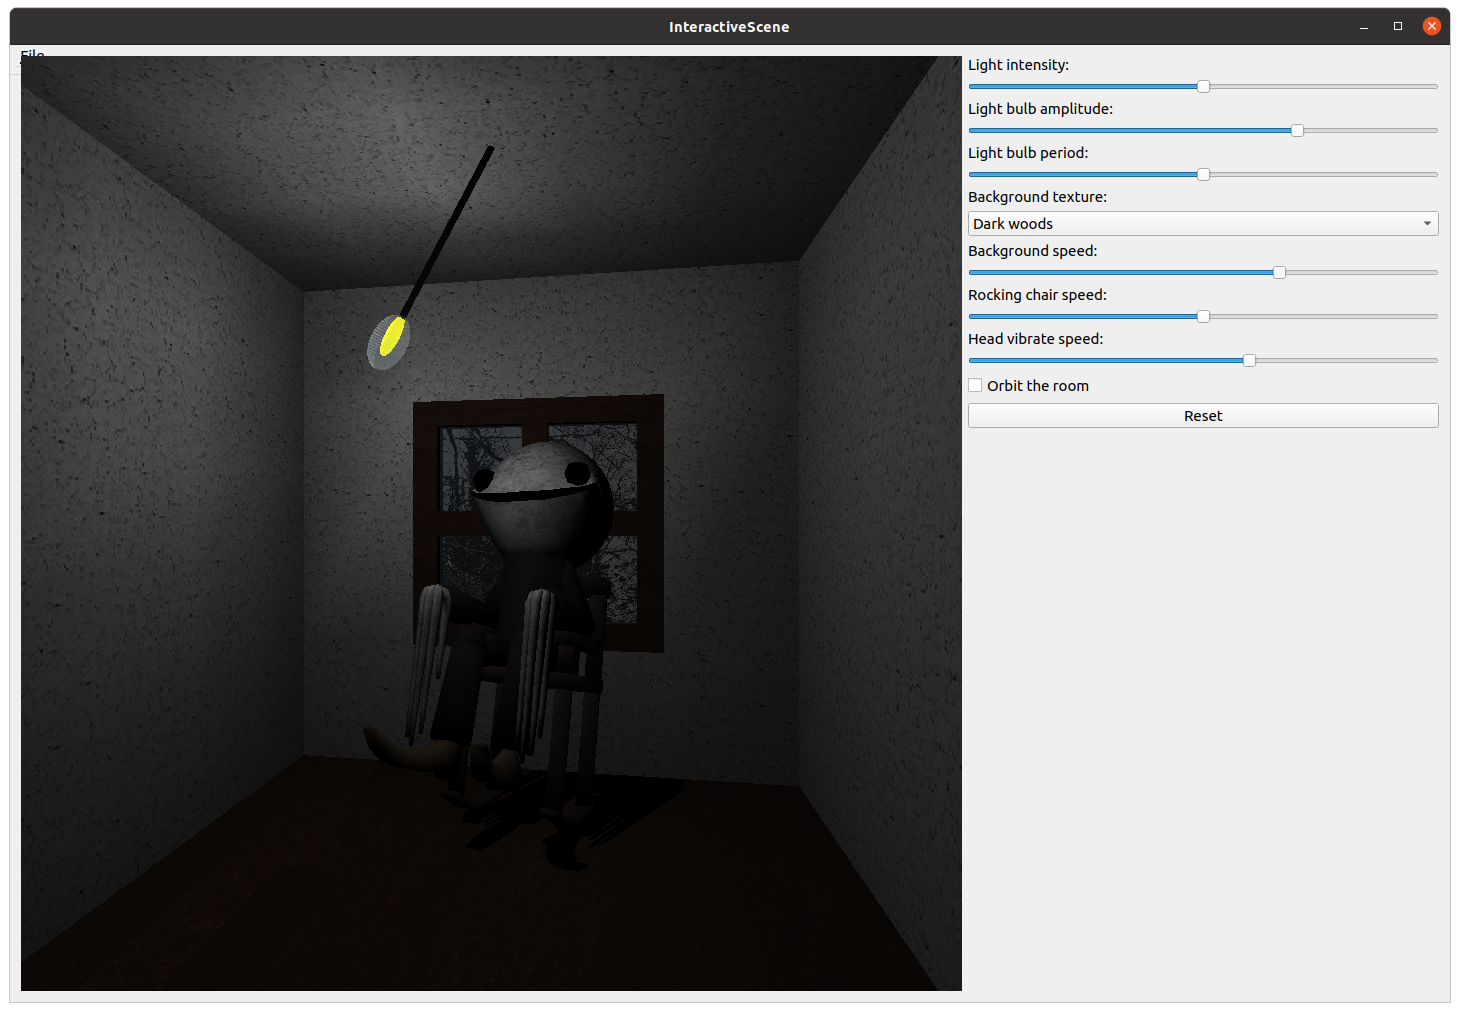
\includegraphics[scale=0.25]{final}
		\caption{Screenshot of the final product}
		\label{final}
	\end{figure}
	\newpage
	\section{Band 4 (40\%-50\%)}
	The requirements of Band 4 are as follows:
	\begin{enumerate}
		\item a visual scene demonstrating reasonable complexity through instancing.
		\item light and material properties that highlight specular and diffusive light contributions.
	\end{enumerate}

	\noindent
	A rough layout of the scene was drawn beforehand to plan for these requirements:
	\begin{figure}[H]
		\centering	
		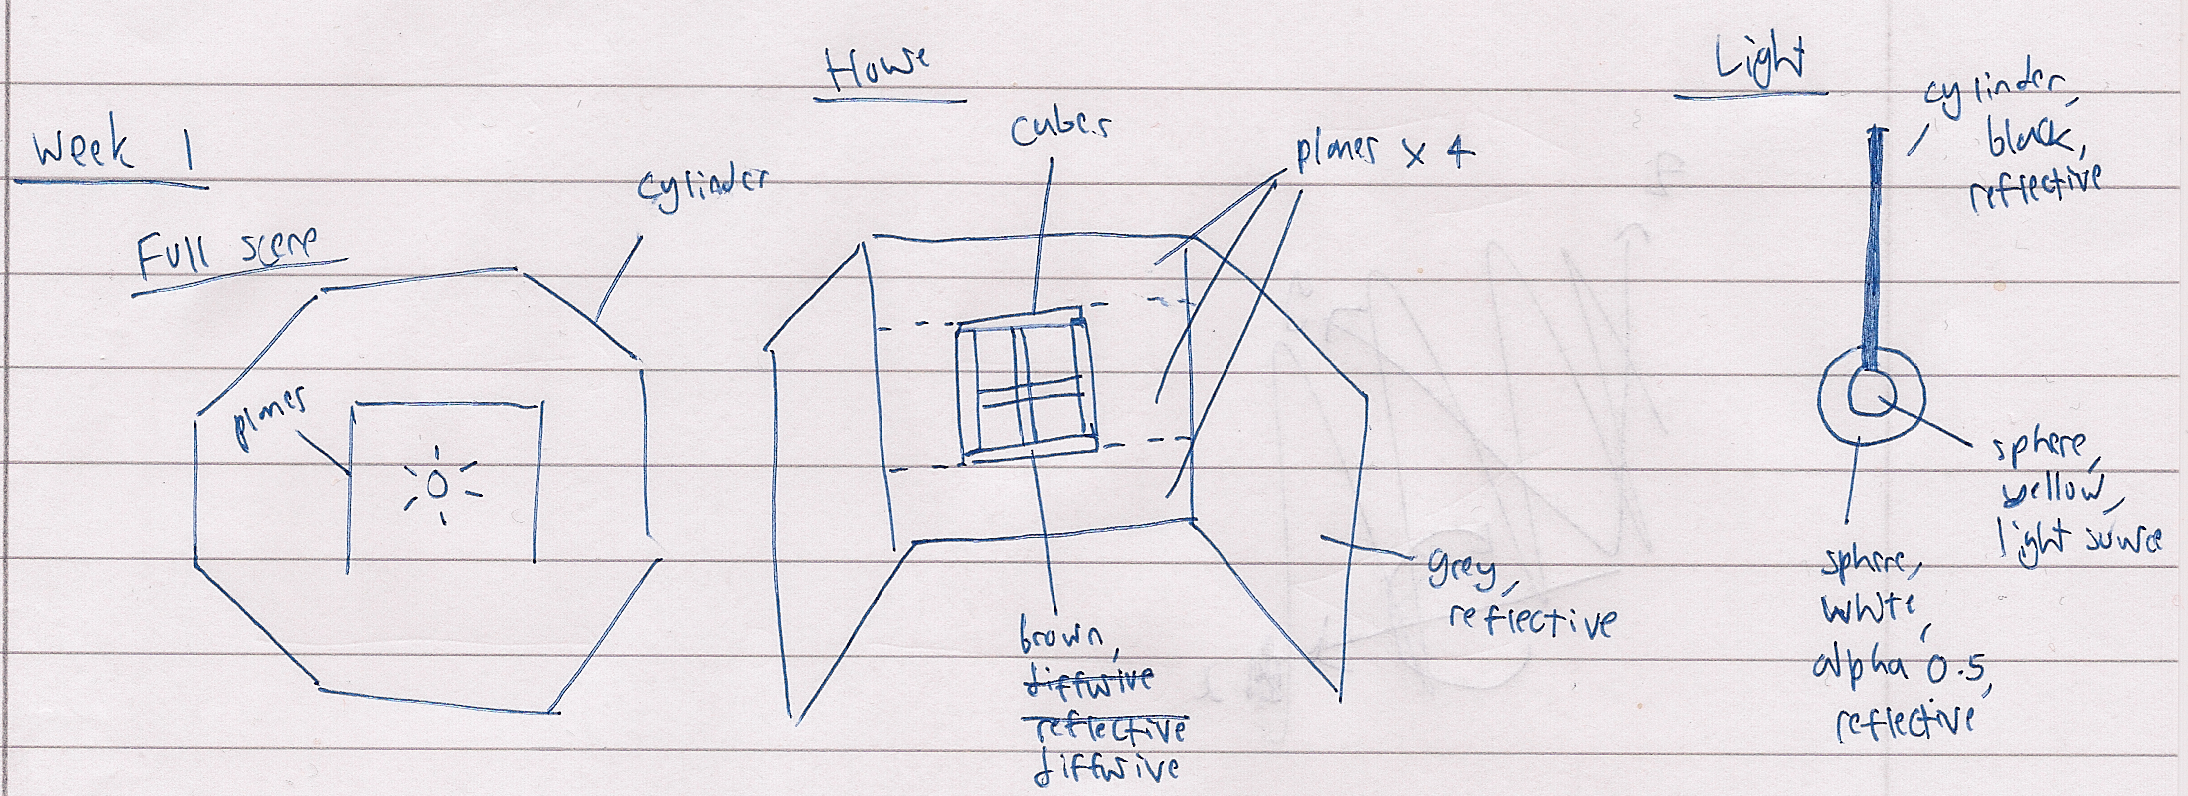
\includegraphics[scale=0.75]{draft-1}
		\caption{Draft of the complex scene}
		\label{draft}
	\end{figure}

		\subsection{Basic objects}
		To facilitate the instantiation of objects in populating our scene, a number of basic
		shapes were defined and implemented as described in Table \ref{shapes}.
		
		\begin{table}[H]
		\begin{tabularx}{\textwidth}{lllX}
		\textbf{Shape} & \textbf{Implementation} & \textbf{Orientation} & \textbf{Description}                                                         \\
		\hline
		square         & GL\_POLYGON             & outside              & tetragon from (0,0,0) to (1,1,0).                                            \\
		cube           & GL\_POLYGON             & outside              & 9 outward-facing squares forming a cube.                                     \\
		cylinder       & GL\_POLYGON             & inside               & taken from COMP3811 tutorials.\newline normals were negated to face inwards. \\
		sphere         & glut object             & inside               & gluSphere with quadric orientation GL\_INSIDE                                                                 
		\end{tabularx}
		\caption{Basic shapes}
		\label{shapes}
		\end{table}

		The choice of shapes was based on the draft
		in Figure \ref{draft}, where cylinders and spheres have their normals pointing inwards as they were designed
		only to contain light sources based on the initial plan.
		The function definitions and the implementation of the square shape can be found in Figures \ref{shapes-h} and
		\ref{square-fn} respectively.

		\noindent
		\begin{figure}
			\centering	
			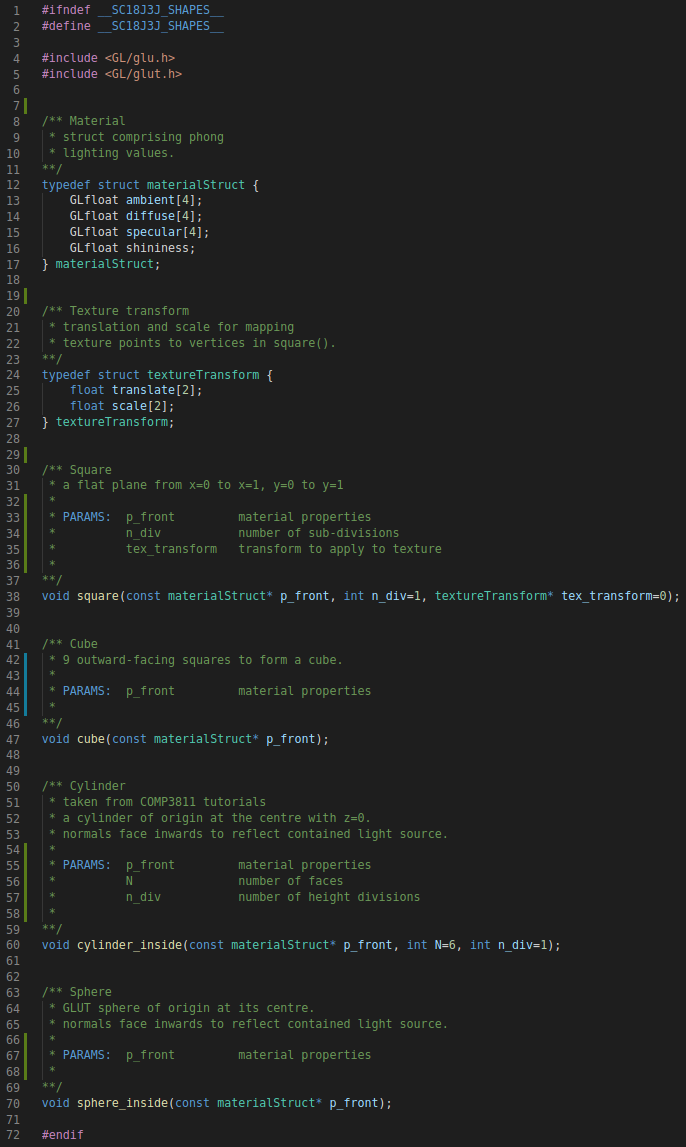
\includegraphics[scale=0.5]{shapes-h}
			\caption{Definitions in \texttt{utils/Shapes.h}}
			\label{shapes-h}
		\end{figure}

		\begin{figure}
			\centering	
			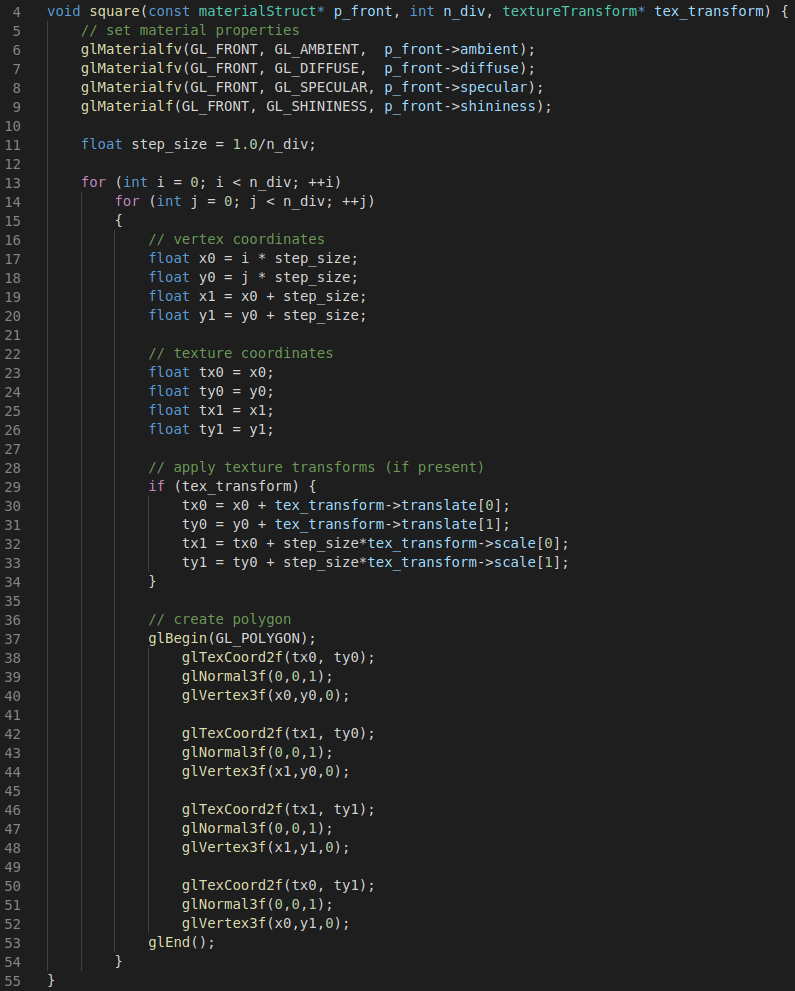
\includegraphics[scale=0.5]{square}
			\caption{\texttt{square()} implementation, \texttt{utils/Shapes.cpp}}
			\label{square-fn}
		\end{figure}

		\subsection{Complex scene}
		The shapes defined in Table \ref{shapes} were successfully instantiated in the scene according
		to the draft in Figure \ref{draft} as illustrated in Figures \ref{scene-ortho} to \ref{scene-persp}.
		Materials defined in Figure \ref{material-predefs} of type \texttt{materialStruct} (Figure \ref{shapes-h})
		were used to accentuate the specular and diffusive lighting provided by OpenGL.

		\bigskip
		
		The code generating the layout of objects in the scene involves a significant number of
		transformations that may be hard to visualise, so the five main segments are described in this section.

		\noindent
		\begin{minipage}{0.5\textwidth}
			\begin{figure}[H]
				\centering	
				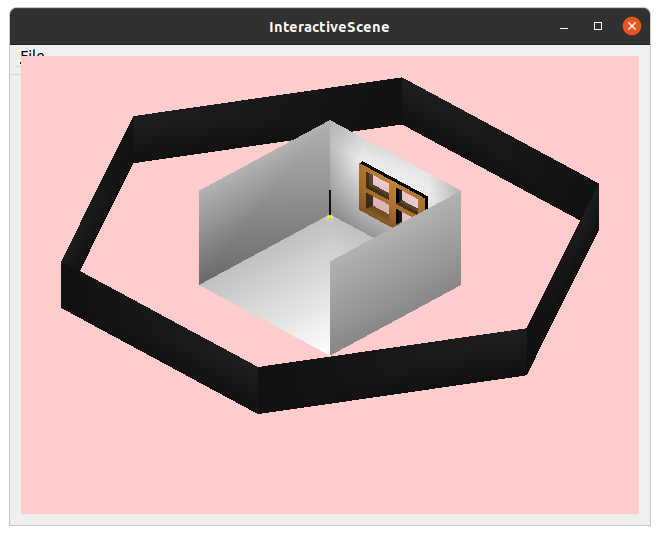
\includegraphics[scale=0.25]{scene-ortho}
				\caption{Orthographic view of complex scene\newline(early implementation)}
				\label{scene-ortho}
			\end{figure}		
		\end{minipage}
		\noindent
		\begin{minipage}{0.5\textwidth}
			\begin{figure}[H]
				\centering	
				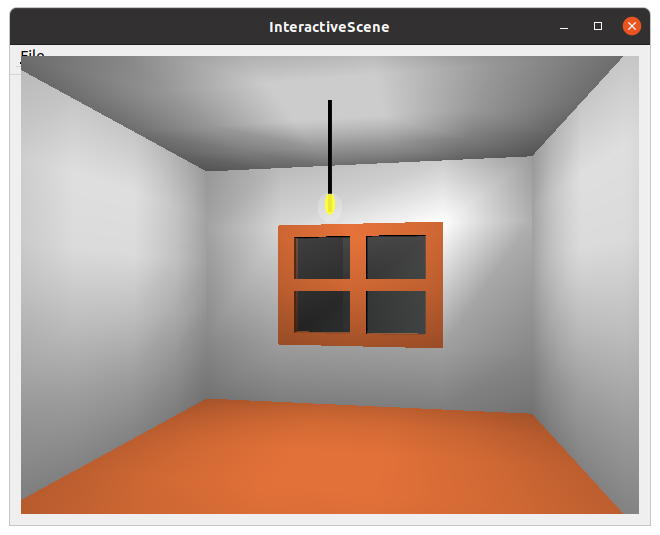
\includegraphics[scale=0.25]{scene-no-atten}
				\caption{Perspective view of complex scene, no light attenuation}
				\label{scene-persp-no-atten}
			\end{figure}		
		\end{minipage}

		\subsubsection{Floor}
		A single instance of \texttt{square()} using the \texttt{woodMaterials} material properties.
		This was later textured with the \texttt{"wild\_cherry\_mysticBrown.png"} image.

		\subsubsection{Walls}
		3 instances of \texttt{square()} for the top, left and right walls. The front wall is comprised of 8
		instances of \texttt{square()} along the sides and diagonals of the window. This is done to
		ensure consistent interpolation of lighting without needing to implement new basic shapes or polygons.
		All of the walls use \texttt{whitePaintMaterials} and were later textured
		with \texttt{"Finishes.Painting.Paint.White.Flaking.jpg"}.

		\subsubsection{Window}
		12 instances of \texttt{cube()}, scaled to cuboids, for the window "bones" and 9 instances of
		\texttt{cube()} for the window "joints". Again, segmentation was done to keep lighting
		consistent. These use the \texttt{woodMaterials} properties, and were later textured with
		the \texttt{"wild\_cherry\_mysticBrown.png"} image. The window panes are a single instance of
		\texttt{square()} using the \texttt{glassMaterials}
		properties, positioned inside of the window frame.

		\subsubsection{Light bulb}
		A single instance of \texttt{cylinder\_inside()} using the \texttt{blackPlasticMaterials}
		properties forms the cable and filament. The glass bulb and yellow light are instances of
		\texttt{sphere\_inside()} using the semi-transparent \texttt{glassMaterials} and
		\texttt{warmLightMaterials} respectively.

		\subsubsection{Background}
		A single instance of \texttt{cylinder\_inside()} using the \texttt{backgroundMaterials} properties,
		giving it high ambient lighting. The texture of this was later implemented to be set via user
		interaction.


		\subsection{Materials and lighting}
		\begin{minipage}{0.5\textwidth}
			\begin{figure}[H]
				\centering
				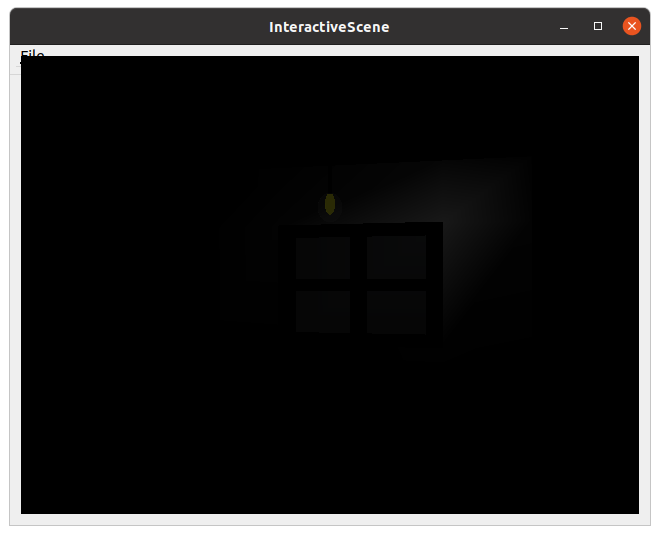
\includegraphics[scale=0.25]{scene-persp-spec}
				\caption{Perspective view of complex scene, specular light only}
				\label{scene-persp-spec}
			\end{figure}		
		\end{minipage}
		\begin{minipage}{0.5\textwidth}
			\begin{figure}[H]
				\centering	
				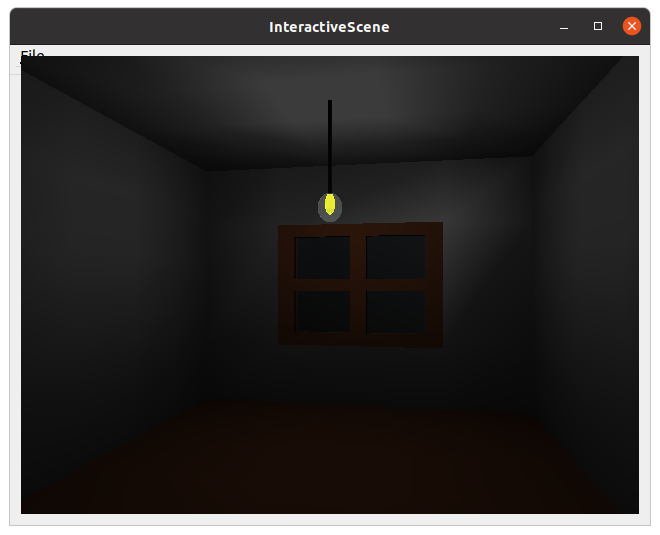
\includegraphics[scale=0.25]{scene-persp}
				\caption{Perspective view of complex scene\newline}
				\label{scene-persp}
			\end{figure}		
		\end{minipage}
		\begin{itemize}
			\item 6 materials of type \texttt{materialStruct} (Figure \ref{shapes-h}) are defined in
			Figure \ref{material-predefs} representing all
			of the materials required for the scene. Most notably, the glass and light materials make use of the alpha channel
			for transparency, while background materials exhibit only ambient light properties.
			\item Alpha blending was used to draw the light bulb and window panes to add transparency and
			create a convincing glass-like appearance.
			\item 2 OpenGL lights are enabled in the scene, namely \texttt{GL\_LIGHT0} to illuminate the room and
			\texttt{GL\_LIGHT1} acting
			as the glow of the light bulb with high attenuation.
			\item Light attenuation was used in favour of spotlights to create a compelling visual atmosphere.
		\end{itemize}

		\begin{figure}[h]
			\centering	
			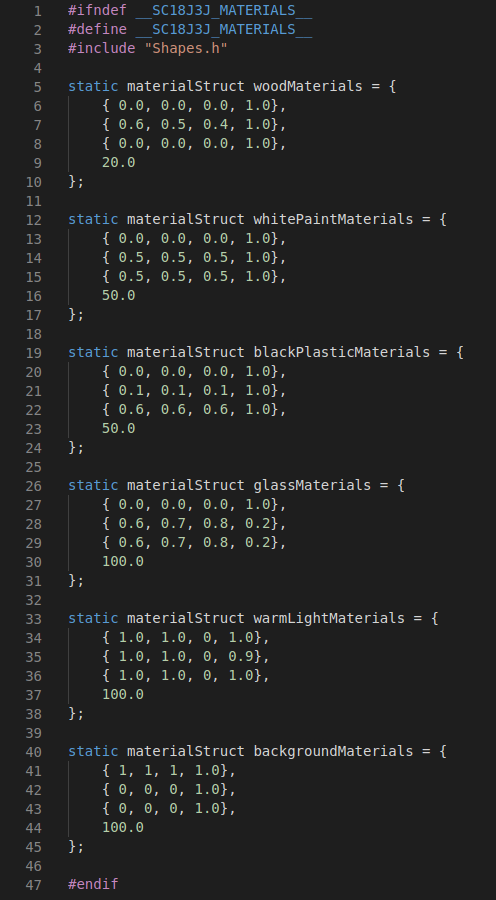
\includegraphics[scale=0.3]{material-predefs}
			\caption{Pre-defined materials in \texttt{utils/MaterialPredefs.h}}
			\label{material-predefs}
		\end{figure}



	\clearpage
	\section{Band 3 (50\%-60\%)}\label{ui}
	The requirements of Band 3 are as follows:
	\begin{enumerate}
		\item The scene contains at least one element of user interaction
	\end{enumerate}
		\subsection{User interaction}
		\begin{table}[H]
		\begin{tabularx}{\textwidth}{|l|l|X|X|}
		\hline
		\textbf{Name}        & \textbf{Type} & \textbf{Values}                                & \textbf{Description}                             \\ \hline
		Light intensity      & QSlider       & range(0,20)                                    & Magnitude of diffuse from light bulb (\texttt{GL\_LIGHT0})\\ \hline
		Light bulb amplitude & QSlider       & range(0,85)                                    & Amplitude of light bulb sine curve               \\ \hline
		Light bulb period    & QSlider       & range(10,30)                                   & Period of light bulb sine curve                  \\ \hline
		Background texture   & QComboBox     & Dark woods/ Marc de Kamps/ Mercator projection & Select background image visible through window   \\ \hline
		Background speed     & QSlider       & range(-6,6)                                    & Speed of background visible through window       \\ \hline
		Rocking chair speed  & QSlider       & range(0,30)                                    & Speed of rocking chair                           \\ \hline
		Head vibrate speed   & QSlider       & range(0,10)                                    & Speed of head vibration                          \\ \hline
		Orbit the room       & QCheckBox     & 0/1                                            & Character will orbit the room if set             \\ \hline
		Reset                & QPushButton   & None                                           & Reset all widgets and geometry to default values \\ \hline
		\end{tabularx}
		\caption{Qt user interface, tabulated}
		\label{ui-table}
		\end{table}

		\begin{figure}[htbp]
			\centering	
			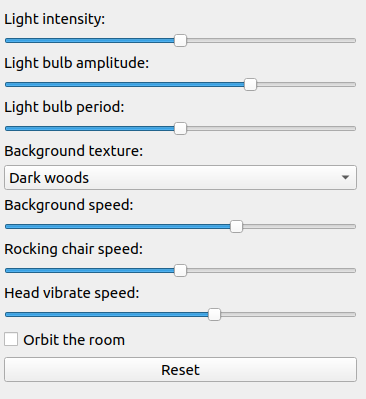
\includegraphics[scale=0.5]{user-interface}
			\caption{Qt user interface, actual}
			\label{ui-actual}
		\end{figure}
		
		\bigskip
		
		User interfaces provided through Qt (Table \ref{ui-table} and Figure \ref{ui-actual}) allow users to change visual aspects of the scene
		including light intensity and the texture of the background visible through the window. Various interfaces are
		also present that control animation described in \ref{animation}, including
		adjustment of the light bulb's sine wave, speed of the background, rocking chair and head,
		as well as setting orbital movement. A \texttt{reset()} function (Figure \ref{default-values}) sets all widgets and
		scene geometry to
		default values, and can be triggered via the "Reset" button.
		
		\bigskip
		
		Signals of each widget are connected to "setter" functions exposed as public slots in the \texttt{QGLWidget}
		such that changes
		in the user interface are almost immediately conveyed to the scene. The setup for this is shown in
		Figures \ref{signal-light} and
		\ref{slot-light} in the case of the light intensity slider, where each widget has a similar implementation.
		
		\bigskip
		
		As illustrated in Figures \ref{signal-light} and \ref{slot-light}, a change in the value of the light intensity 
		slider will emit a signal to the corresponding slot in the \texttt{QGLWidget}, which in turn directly sets the
		diffuse property of \texttt{GL\_LIGHT0}.
		
		\bigskip
		
		\begin{figure}[htbp]
			\centering	
			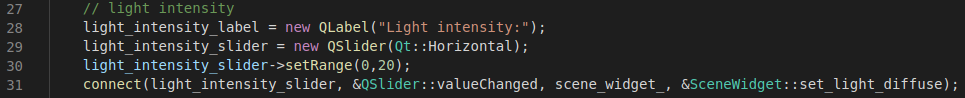
\includegraphics[scale=0.5]{signal-light}
			\caption{Setup of light intensity slider, \texttt{MainWindow.cpp}}
			\label{signal-light}
		\end{figure}
		\begin{figure}[htbp]
			\centering	
			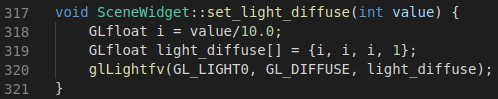
\includegraphics[scale=0.5]{slot-light}
			\caption{Implementation of light intensity slot, \texttt{MainWindow.cpp}}
			\label{slot-light}
		\end{figure}
		\begin{figure}[htbp]
			\centering	
			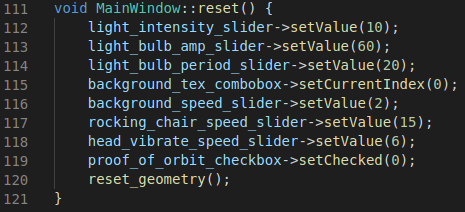
\includegraphics[scale=0.5]{default-values}
			\caption{Implementation of \texttt{reset()}, \texttt{MainWindow.cpp}}
			\label{default-values}
		\end{figure}




	\clearpage
	\section{Band 2 (60\%-70\%)}
		The requirements of Band 2 are as follows:
		\begin{itemize}
			\item an element of animation
			\item one convex object constructed from polygons
			\item texture mapping
		\end{itemize}
		\subsection{Animation}\label{animation}
			Animation is created in the scene through a series of transformations over time. The \texttt{QGLWidget} rendering
			the scene is updated by a \texttt{QTimer} in the main window, aiming for a refresh rate of 100 frames per second.
			At each update, calculations are performed that adjust the transformations of objects to simulate movement
			in the scene (Figure \ref{update-angles}). 2 variations of movement were implemented for this project as described below.
			
			\bigskip

			\begin{figure}[h]
			\centering	
			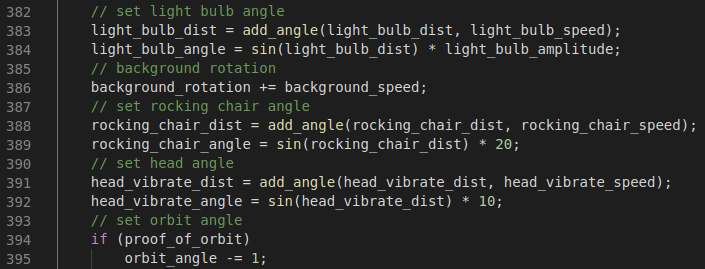
\includegraphics[scale=0.3]{update-angles}
			\caption{Distance and angle calculations performed on frame update, \texttt{SceneWidget.cpp}}
			\label{update-angles}
			\end{figure}

			\subsubsection{Oscillation}
			Sine waves were used to animate oscillation in the OpenGL lights \texttt{GL\_LIGHT0} and \texttt{GL\_LIGHT1} and the
			light bulb object, creating the effect of a swinging light source. Sine waves were also used to
			generate oscillation in the character's rocking chair and head.
			
			\bigskip
			
			Oscillating objects are given a speed, where their angle of rotation at a given frame is a
			function of the distance travelled represented by a sine wave. All distances are updated
			at each frame update, and are normalised
			between the range of $-2\pi$ to $2\pi$ before they are passed to the sine function.

			\bigskip
						
			As an example, the plot of the
			light bulb angle as a function of distance using the default amplitude and period is shown in
			Figure \ref{light-curve}.

			\begin{figure}[H]
				\centering	
				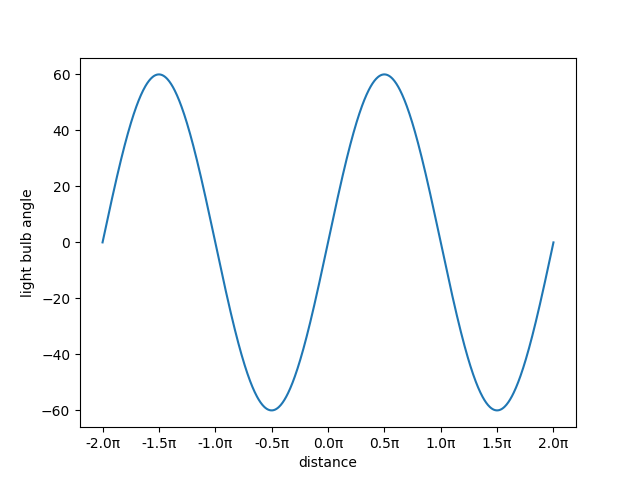
\includegraphics[scale=0.5]{light-curve}
				\caption{Light bulb angle as a function of distance}
				\label{light-curve}
			\end{figure}
			
			
			\subsubsection{Orbit}
			To animate an orbital motion around the room, we start at the centre point (0,0,0) and rotate by
			the orbit angle $\theta$ degrees in the z-axis. We then translate to (0,0.25,0) and draw the
			character.
			The orbit angle $\theta$ is decremented on each frame update if the QCheckBox 
			labelled "Orbit the room" is set by the user. This creates circular movement in
			the clockwise direction around the scene. The background cylinder orbits the room in a similar manner,
			albeit without any translation.

			\bigskip

			\begin{figure}[H]
				\centering	
				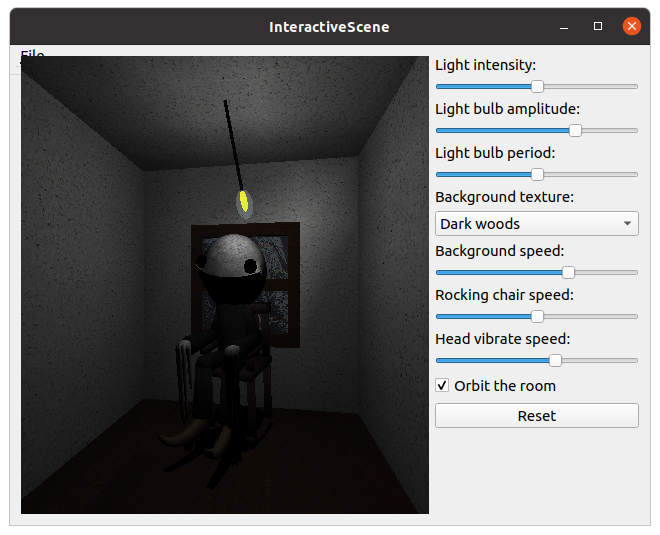
\includegraphics[trim=20 20 230 60, clip, scale=0.15]{anim-0}
				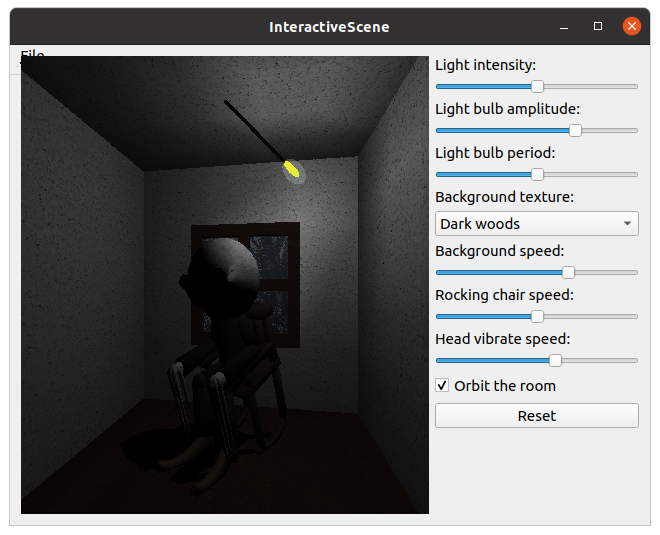
\includegraphics[trim=20 20 230 60, clip, scale=0.15]{anim-1}
				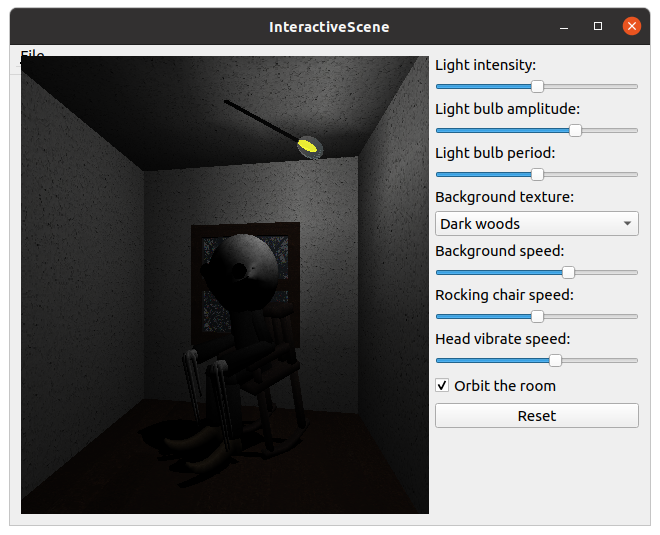
\includegraphics[trim=20 20 230 60, clip, scale=0.15]{anim-2}
				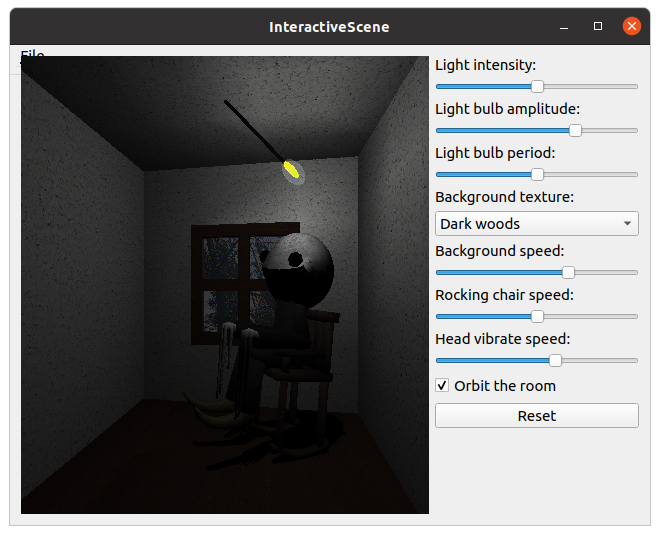
\includegraphics[trim=20 20 230 60, clip, scale=0.15]{anim-3}
				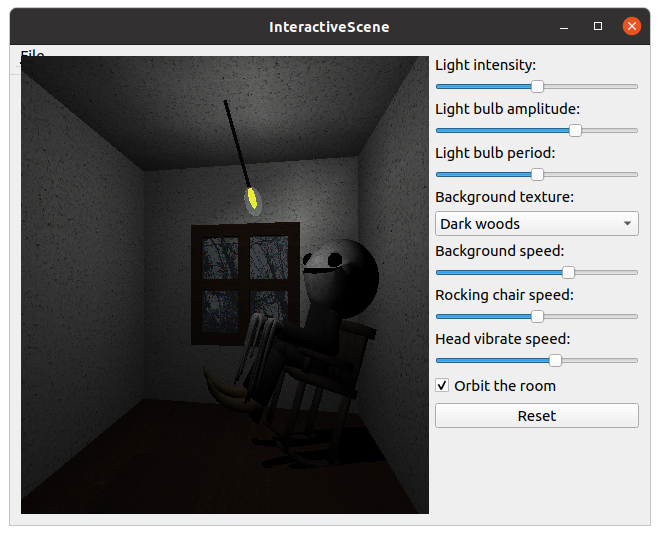
\includegraphics[trim=20 20 230 60, clip, scale=0.15]{anim-4}
				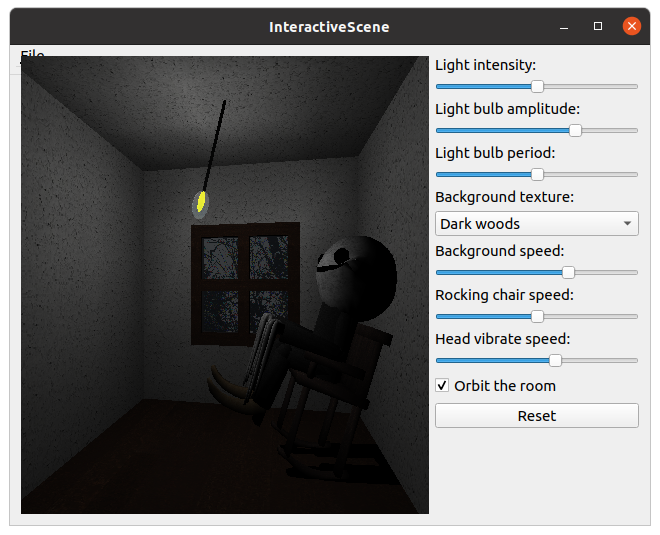
\includegraphics[trim=20 20 230 60, clip, scale=0.15]{anim-5}
				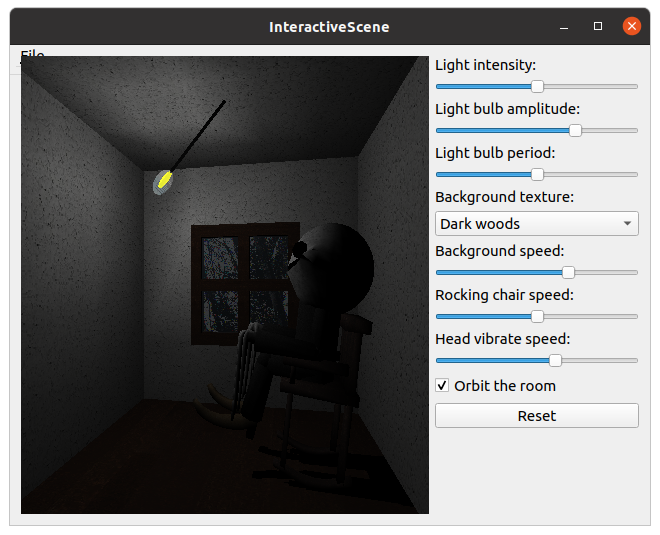
\includegraphics[trim=20 20 230 60, clip, scale=0.15]{anim-6}
				\caption{Animation in the scene (left to right)}
				\label{anim-reel}
			\end{figure}

		\subsection{Convex objects}\label{convex-object}
		A long-standing personal goal of mine is to learn how to create 3D art.
		This lined up nicely with the requirements of Band 2, and a convex object constructed from
		polygons was modelled using 3DS Max for the scene.
		
		\bigskip
		
		While most of the model is made up of basic convex shapes, complex geometry in the hands, face, shoes and
		rocking chair required the manipulation and creation of individual polygons which can be seen in the workspace view
		in Figure \ref{workspace}.
		
		\begin{figure}[htbp]
			\centering	
			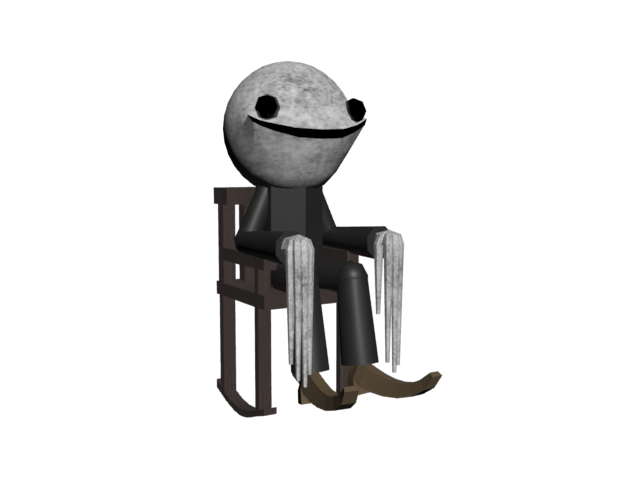
\includegraphics[scale=0.5]{character}
			\caption{Render of our convex object}
			\label{character}
		\end{figure}
		\begin{figure}[htbp]
			\centering	
			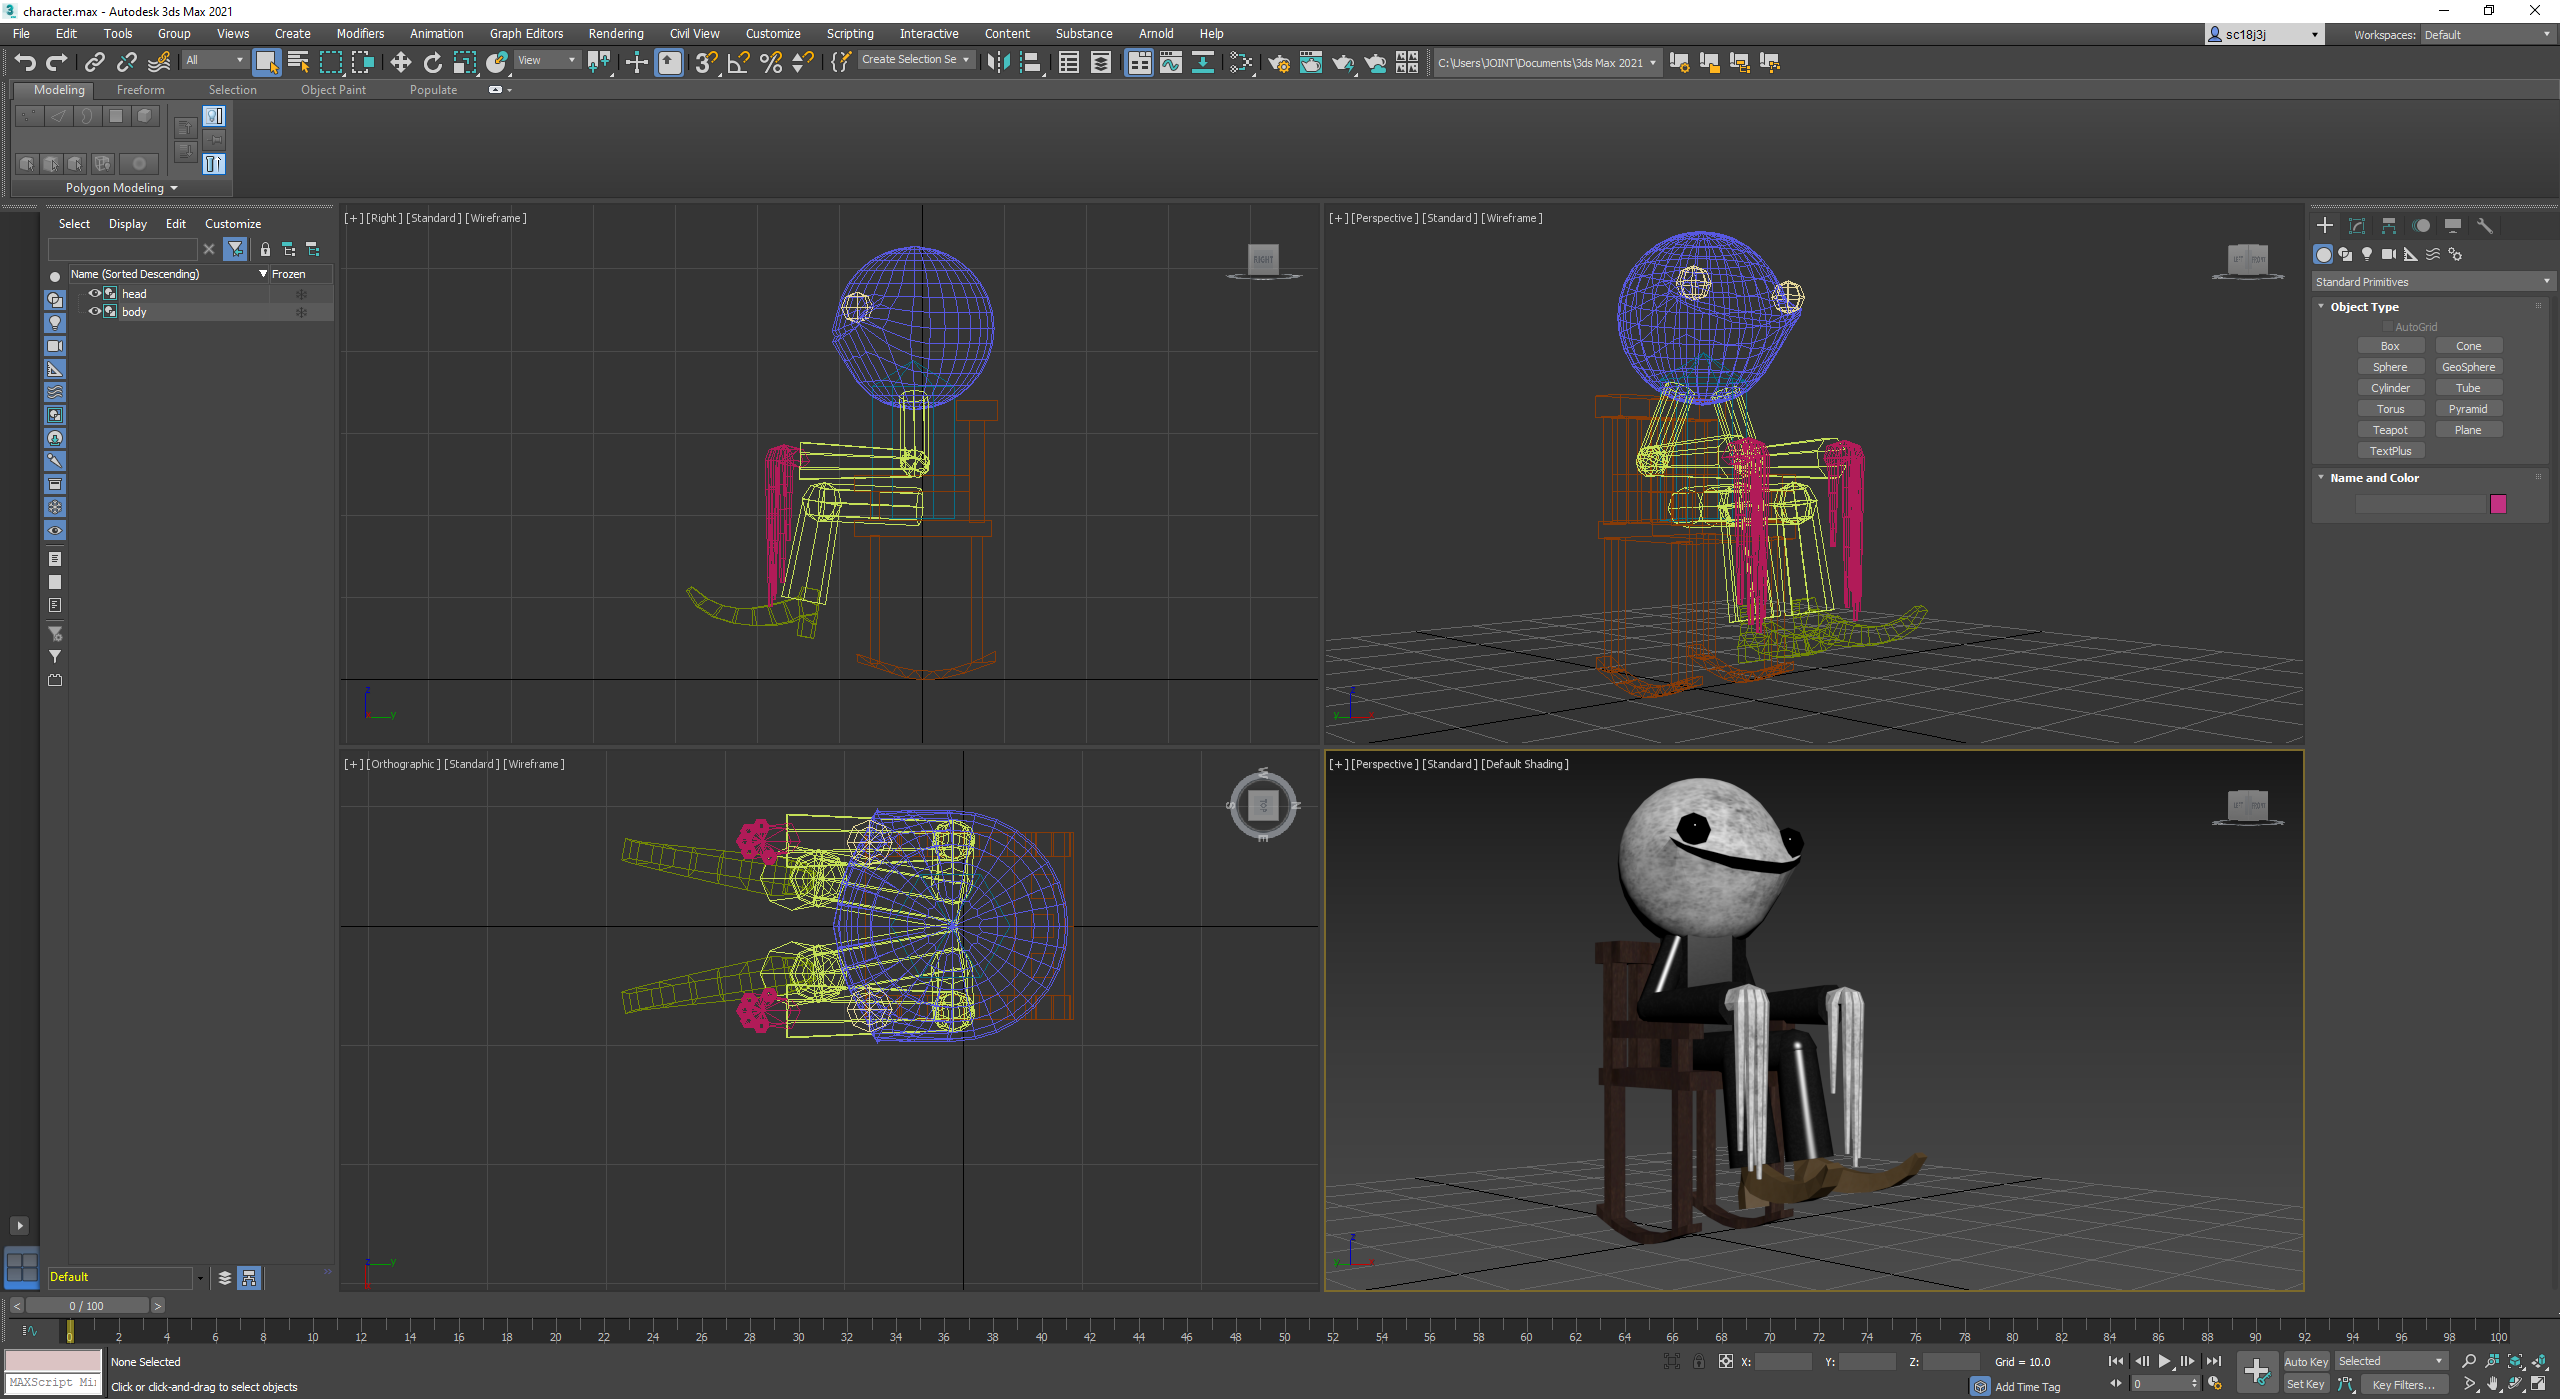
\includegraphics[scale=0.25]{workspace}
			\caption{Workspace view of our convex object highlighting individual polygons}
			\label{workspace}
		\end{figure}

		The head and body were exported separately in the Wavefront \texttt{.obj} format, and a \texttt{wavefrontObj} class
		was implemented in C++ to parse the files and draw their corresponding objects using OpenGL.
		
		\bigskip
		
		The \texttt{wavefrontObj} class implements 3 main functions, namely \texttt{draw()}, \texttt{load()} and
		\texttt{load\_mtl()}. \texttt{draw()} handles the instantiation of the object in the scene, loading texture and
		material properties before emitting OpenGL vertex, normal and texture coordinates for each polygon
		(Figure \ref{obj-draw}). \texttt{load()} and \texttt{load\_mtl()} parse input \texttt{.obj} and \texttt{.mtl} files
		and store the material, texture and coordinate information required by \texttt{draw()}.
		
		\bigskip
		
		An example of parsing a vertex
		is shown in Figure \ref{parse-vert}, where other information such as texture coordinates and material definitions
		are processed in a similar manner over a loop on every line in the input file.
		
		\bigskip
		
		On a side note, the definition of \texttt{cube()} in Figure \ref{shapes-h} constitutes a convex object constructed from
		polygons, as it forms a solid cube from 9 instances of \texttt{square()}, which are themselves polygons created in OpenGL.

			\begin{figure}[h]
				\centering	
				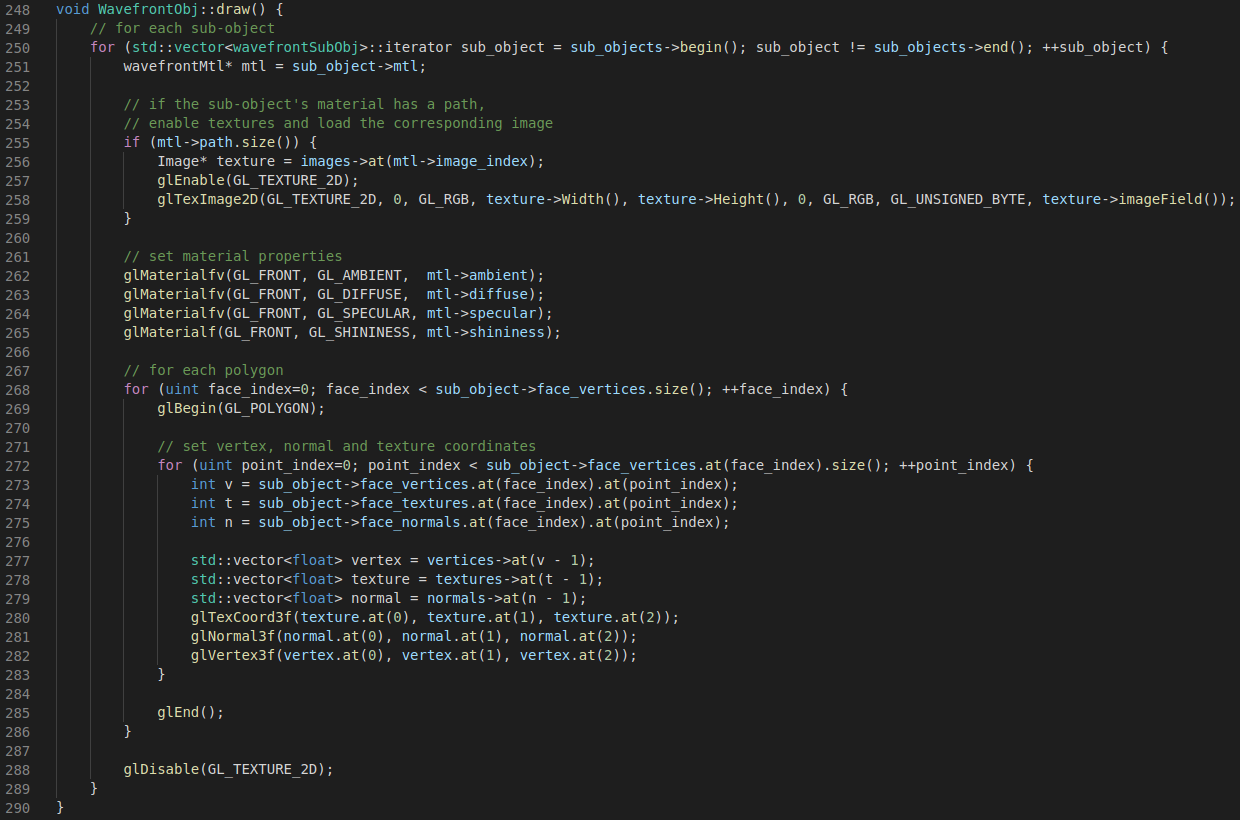
\includegraphics[scale=0.3]{obj-draw}
				\caption{Implementation of \texttt{wavefrontObj::draw()}, \texttt{utils/WavefrontObj.cpp}}
				\label{obj-draw}
			\end{figure}
			\begin{figure}[h]
				\centering	
				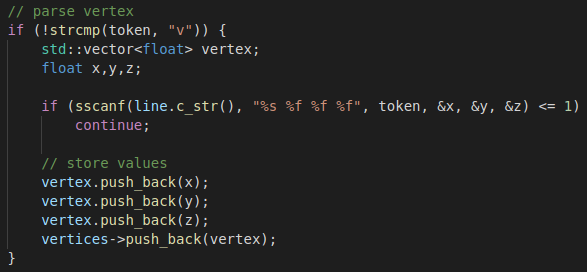
\includegraphics[scale=0.35]{parse-vertex}
				\caption{Implementation of parsing a vertices in a \texttt{.obj} file, \texttt{utils/WavefrontObj.cpp}}
				\label{parse-vert}
			\end{figure}

		\subsection{Texture mapping}
		The implementation of texture mapping in the scene is shown in
		Figures \ref{shapes-h}, \ref{square-fn} and \ref{obj-draw}. Images are loaded into the application using
		the \texttt{Image} class
		provided in the COMP3811 tutorials, and set in OpenGL with \texttt{glTexImage2D()}.
		
		\bigskip
		
		Instances of \texttt{square()} map the entire image to the polygon face of the square, subject to
		transformations specified by the \texttt{textureTransform} struct defined in Figure \ref{shapes-h}.
		The transform scales and offsets the image by a user-specified value to allow for a continuous image
		across multiple textured instances of \texttt{square()}.

		\bigskip

		Instances of \texttt{cylinder()} simply map the entire image to each polygon face of the cylinder.
		
		\bigskip
		
		Finally, texture mapping is performed on imported \texttt{.obj} models using texture information
		parsed from input files. Each sub-object in a \texttt{.obj} file can specify an image, stored
		in a \texttt{.mtl} file, and texture coordinates for each polygon vertex. As such, we simply load the
		corresponding image for each sub-object and emit the texture and vertex coordinates for each polygon to
		draw a textured 3D model.

		\begin{minipage}{0.5\textwidth}
			\begin{figure}[H]
				\centering	
				
\includegraphics[scale=0.1]{Finishes.Painting.Paint.White.Flaking}
				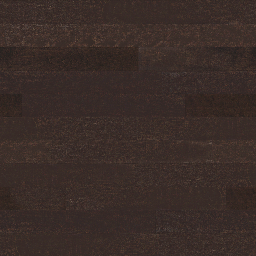
\includegraphics[scale=0.1]{wild_cherry_mysticBrown}
				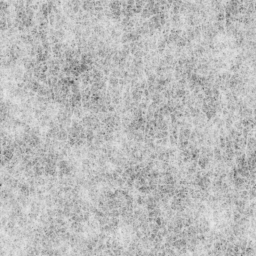
\includegraphics[scale=0.25]{leather_aged_rough}
				
\includegraphics[scale=0.45]{Furnishings.Fabrics.Velvet.Black}
				
\includegraphics[scale=0.2]{Furnishings.Fabrics.Leather.Pebble.Brown}
				\caption{Autodesk textures}
				\label{autodesk-tex}
			\end{figure}
		\end{minipage}
		\begin{minipage}{0.5\textwidth}
			\begin{figure}[H]
				\centering	
				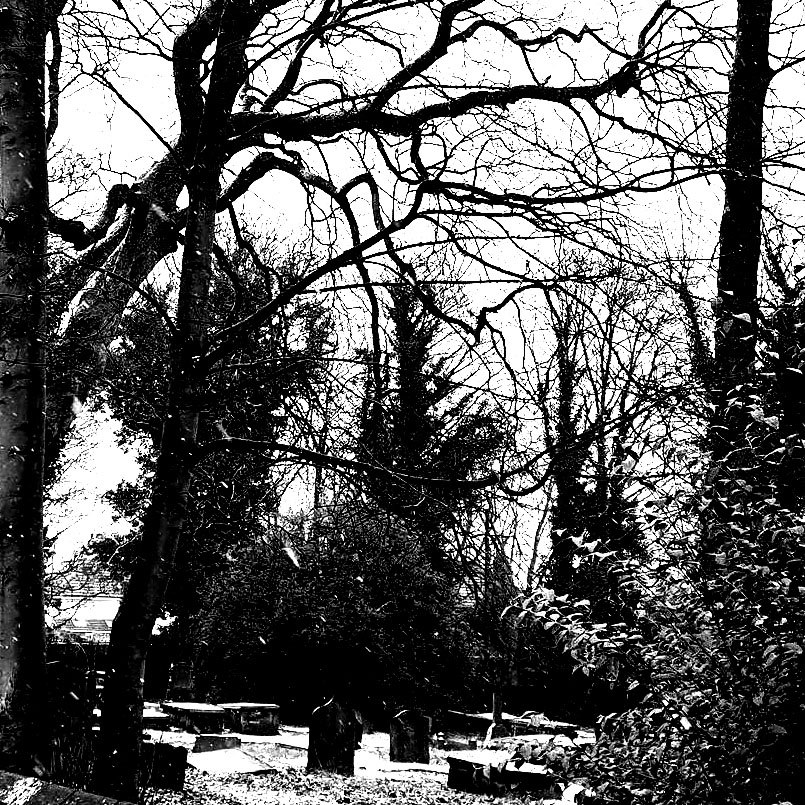
\includegraphics[scale=0.25]{dark_woods}
				\caption{Dark woods texture, photographed in Chapel Allerton}
				\label{dark-woods}
			\end{figure}
		\end{minipage}

		\begin{figure}[H]
			\centering	
			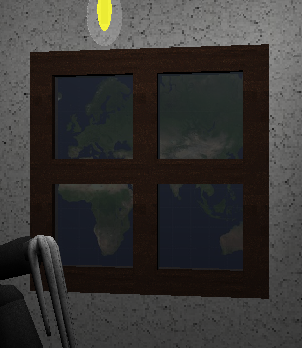
\includegraphics[scale=0.7]{window}
			\caption{Background texture visible through window}
			\label{bg-texture}
		\end{figure}

		A number of images were introduced to texture different elements of the scene.
		The images shown in Figure \ref{autodesk-tex} were taken from the default material library included with 3DS Max.
		
		\bigskip
		
		The image of Dr Marc de Kamps and the Mercator Projection were
		used as background textures visible through the window of the scene (Figure \ref{bg-texture}),
		with an additional photograph taken in Leeds (Figure \ref{dark-woods}) with the intention of adding
		to the visual atmosphere.
		
		\bigskip
		
		The choice of background image in the scene can be made via the user interface detailed
		in section \ref{ui}, with the code that loads the selected image shown in Figure \ref{texture-bg}.
		
		\bigskip
		
		\begin{figure}[H]
			\centering	
			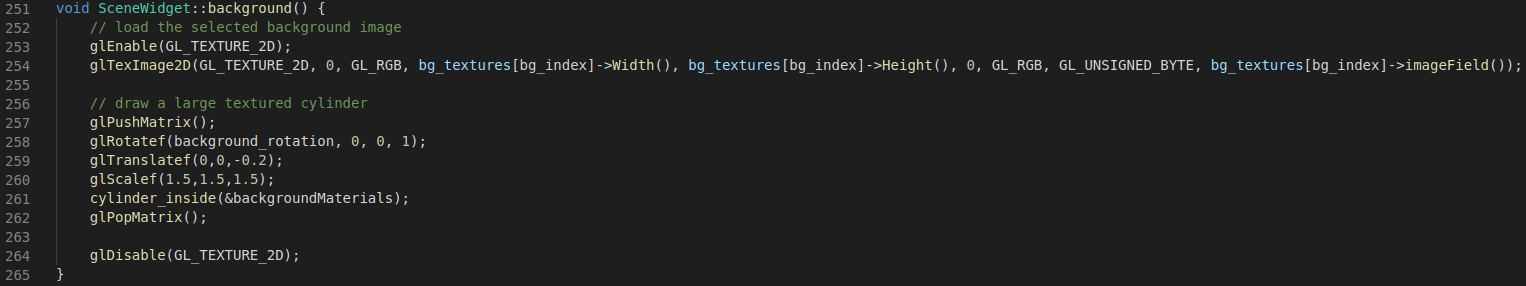
\includegraphics[scale=0.3]{texture-bg}
			\caption{Loading the background texture image in \texttt{SceneWidget.cpp}}
			\label{texture-bg}
		\end{figure}



	\clearpage
	\section{Band 1 (70\%-100\%)}
		The requirements of Band 1 are as follows:
		\begin{itemize}
			\item The scene contains an object that requires hierarchical modelling and displays motion in some of its parts.
			\item Various elements of user interaction are used.
		\end{itemize}
		\subsection{Hierarchical modelling}\label{hier}
		As explained in section \ref{convex-object} our character was exported in two parts,
		namely its head and body. This allows us to perform hierarchical modelling where the head and the body
		can be drawn as children of the character instance, with their pose dependent on that of the parent.
		
		\bigskip
		
		This is shown clearly through animation, where the character can be set to orbit around the room while
		its entire body rocks with its head rotating in place. All of this is seen
		to occur without changing the relative position of the head to the character origin as a result of
		hierarchical modelling.

		\noindent
		\begin{minipage}{\textwidth}
			\begin{figure}[H]
				\centering	
				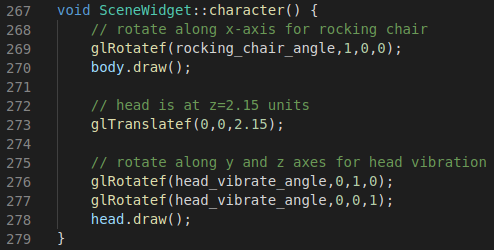
\includegraphics[scale=0.5]{hierarchical}
				\caption{Hierarchical implementation of the character object in \texttt{SceneWidget.cpp}}
				\label{hierarchical}
			\end{figure}
		\end{minipage}
		
		\bigskip
		The implementations of \texttt{cube()} and \texttt{house()} also make use of hierarchical modelling,
		where the former creates a convex object out of multiple squares, and the latter creates a complex scene
		using a variety of basic shapes, all relative to the origin of the instance.
		
		\subsection{User interaction}
		Users are able to interact with the hierarchical model by setting the head vibration speed, rocking chair speed and
		its orbit around the room using the interfaces outlined in section \ref{ui}. Sections \ref{animation} 
		and \ref{hier} detail the process of animating these movements in the character.

		\subsection{Shadow implementation}
		Without the use of a shader, we model shadows in the scene by applying transformations to the model-view
		matrix that shear and flatten objects drawn onto the scene.
		
		\bigskip
		
		Setting the z coordinate to 0 in the model-view matrix flattens the z-axis, allowing us
		to draw on a 2D plane where z=0.

		\bigskip

		A positive z-shear in the x-axis draws the shadow to the left of the character, while a negative z-shear
		in the x-axis draws it to the right. Similarly, a positive z-shear in the y-axis draws the shadow
		behind the character, while a negative z-shear in the y-axis draws it in front.
		
		\bigskip
		
		We can thus model the direction of the shadow given the state of the scene, using sine
		and cosine  waves to estimate the length of the z-shear in both axes from the character's
		position along its orbit in relation to the light source, and sine waves to approximate z-shear in the
		y-axis from rotation of the rocking chair.

		\noindent
		\begin{minipage}{\textwidth}
			\begin{figure}[H]
				\centering	
				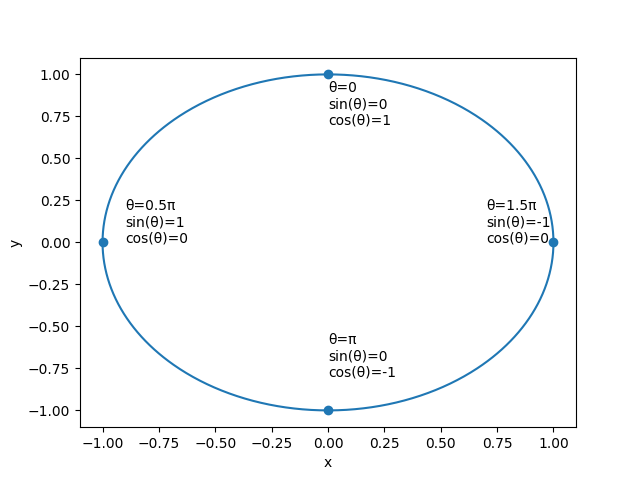
\includegraphics[scale=0.5]{orbit-waves}
				\caption{Plot of character orbit labelled with orbit angle $\theta$ (normalised) in radians.}
				\label{orbit-waves}
			\end{figure}
		\end{minipage}

		\bigskip
				
		The computed z-shears and flattening effect mentioned above are combined into a single matrix to form
		our shadow transformation matrix. We apply this transformation to the model-view matrix, temporarily
		disable depth testing and lighting and set the colour to (0,0,0,1) before drawing our character model.
		This has the effect of generating a flat dark shadow of the character on the floor where z=0.
		
		\bigskip
		
		The code for calculating the shadow transform can be found in Figure \ref{shadow-code}, while Figure \ref{shadow-reel}
		features some interesting shadows generated from this effect.
		
		\bigskip

		\begin{figure}[H]
			\centering	
			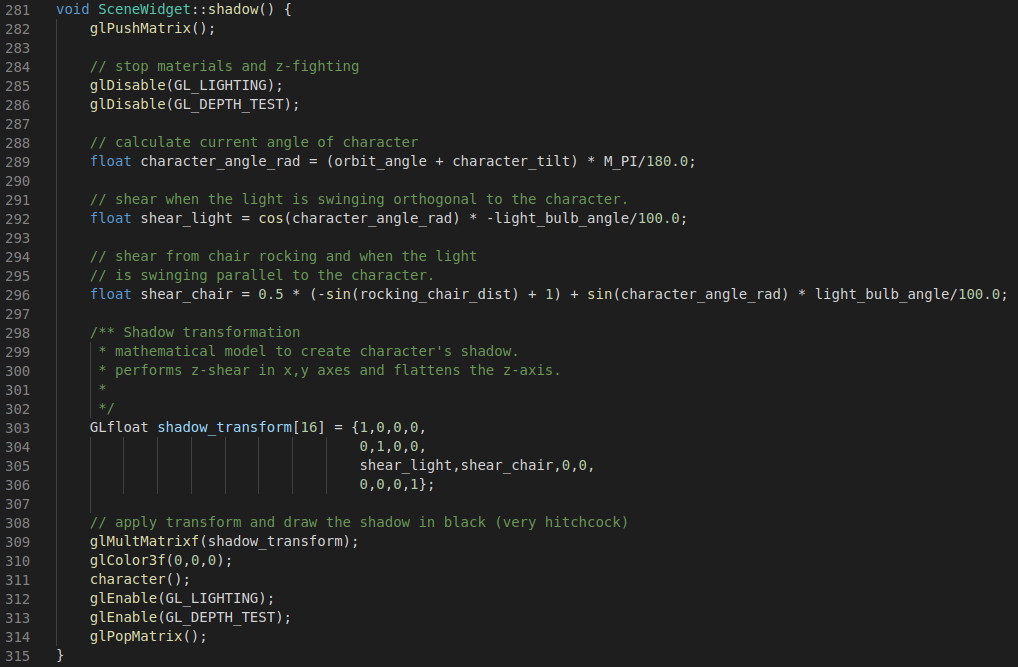
\includegraphics[scale=0.35]{shadow-code}
			\caption{implementation of shadows in \texttt{SceneWidget.cpp}}
			\label{shadow-code}
		\end{figure}
		
		\begin{figure}[H]
			\centering	
			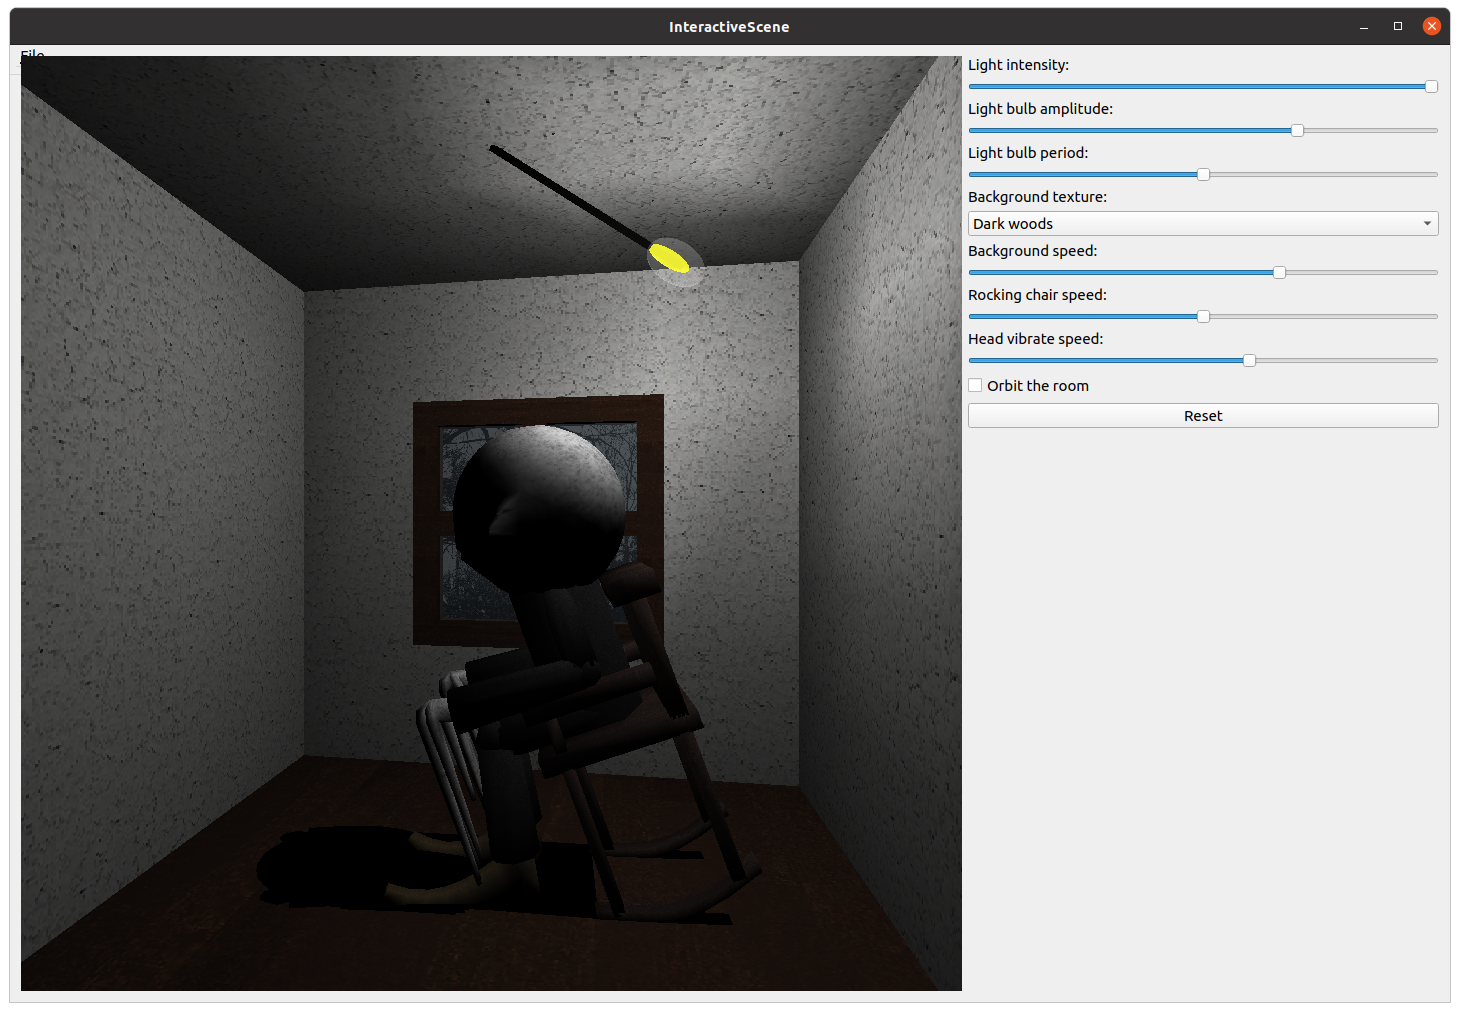
\includegraphics[trim=20 20 500 60, clip, scale=0.2]{shadow-1}
			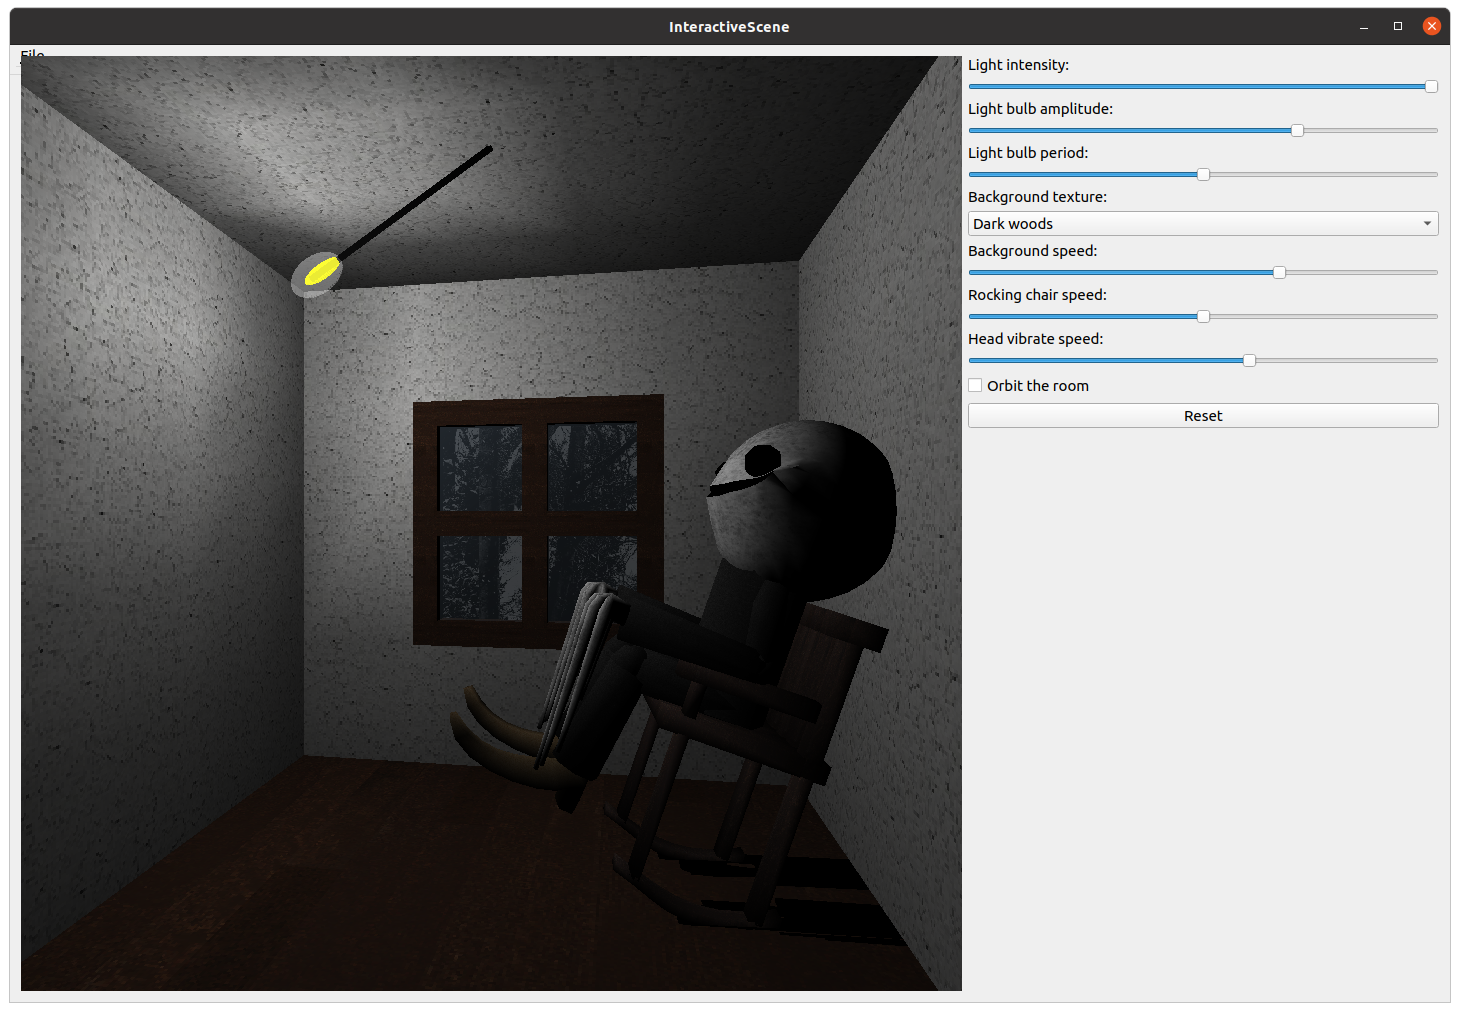
\includegraphics[trim=20 20 500 60, clip, scale=0.2]{shadow-2}
			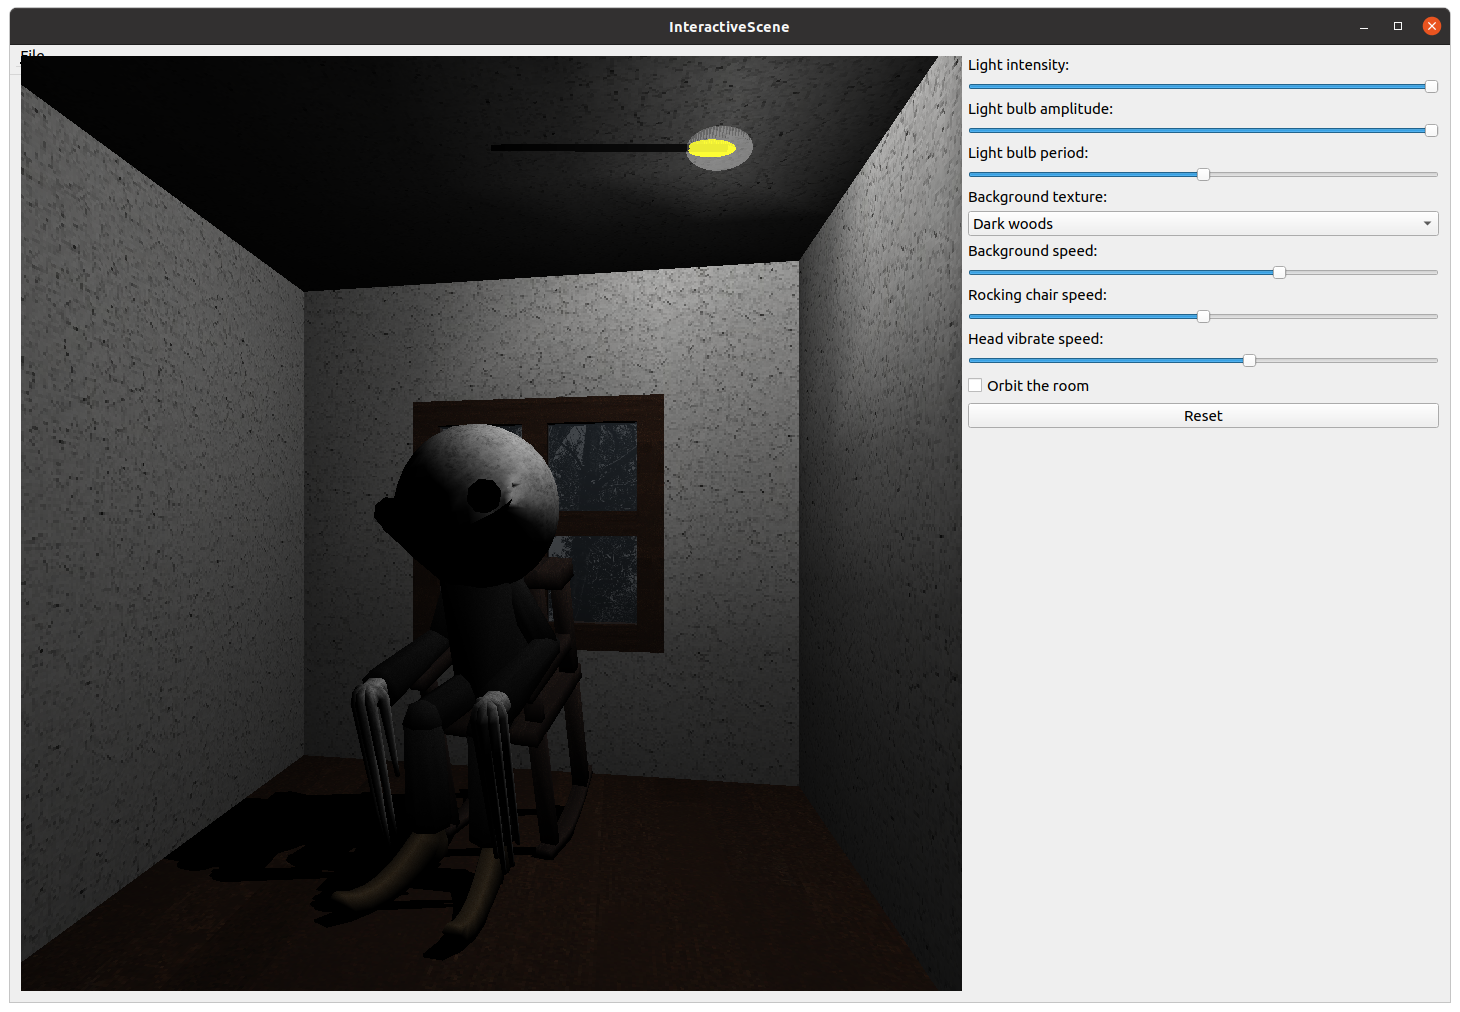
\includegraphics[trim=20 20 500 60, clip, scale=0.2]{shadow-3}
			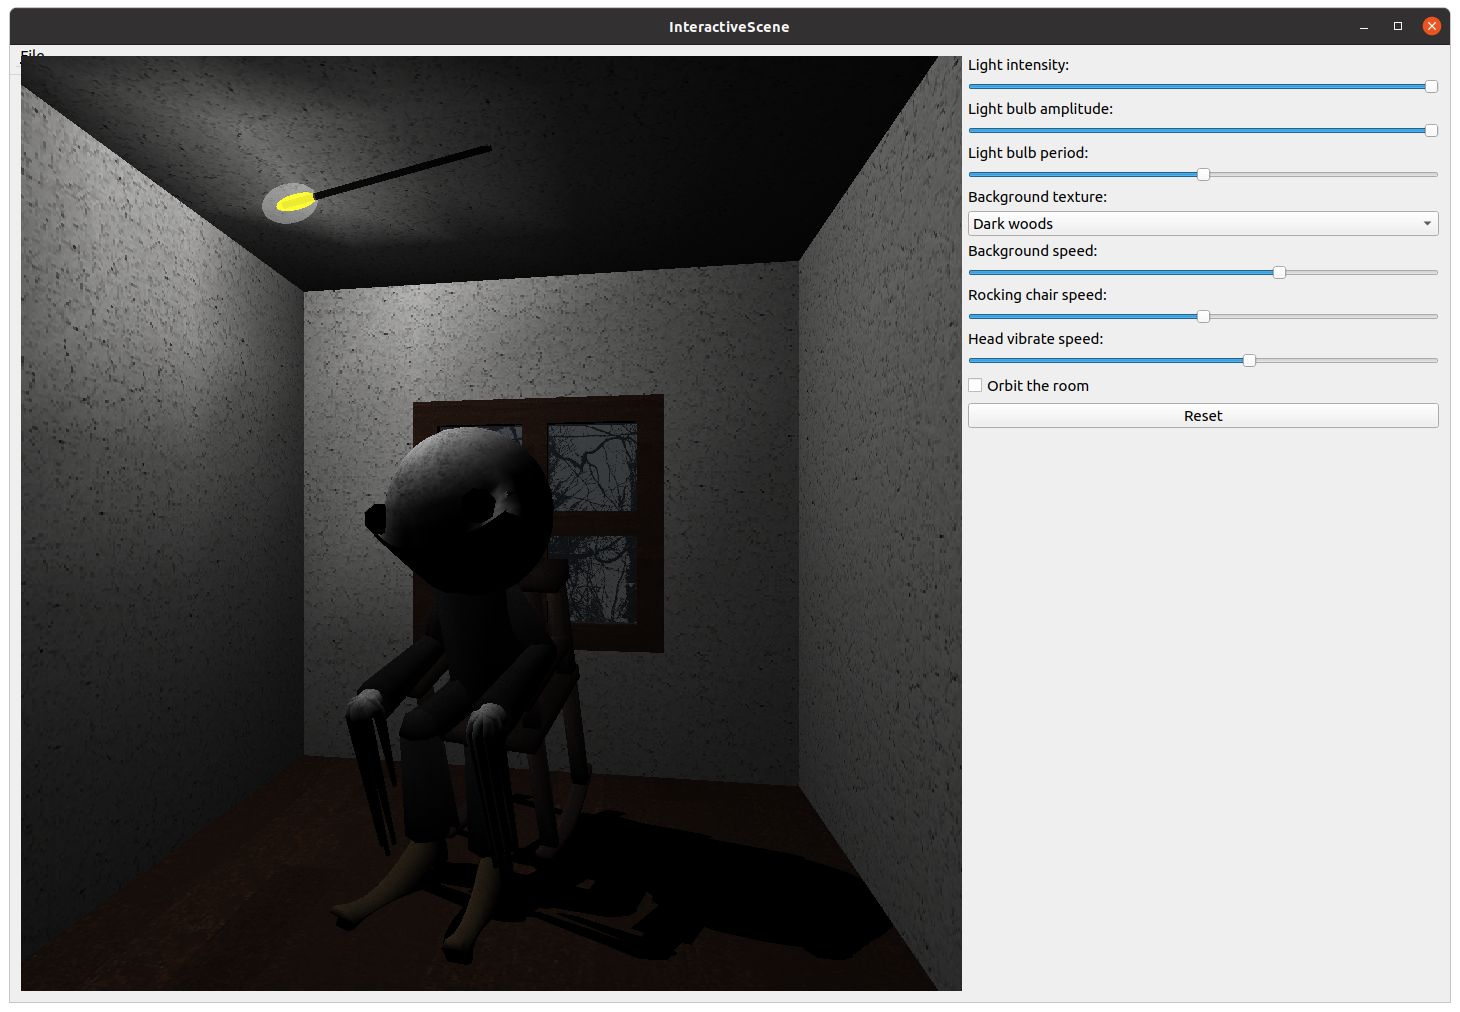
\includegraphics[trim=20 20 500 60, clip, scale=0.2]{shadow-4}
			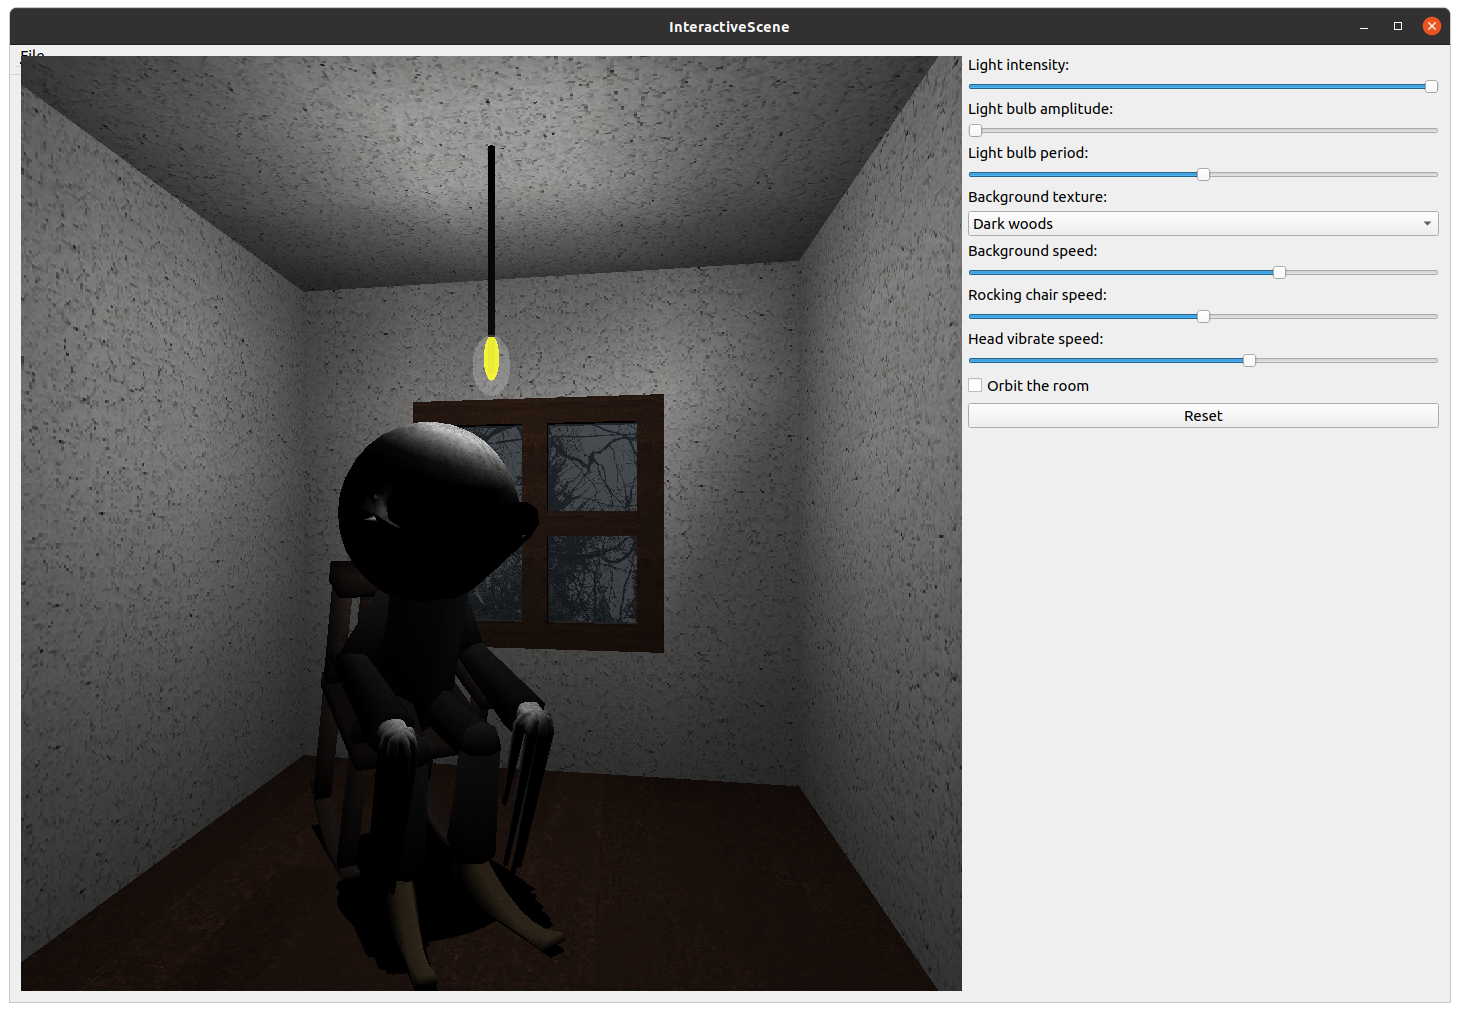
\includegraphics[trim=20 20 500 60, clip, scale=0.2]{shadow-5}
			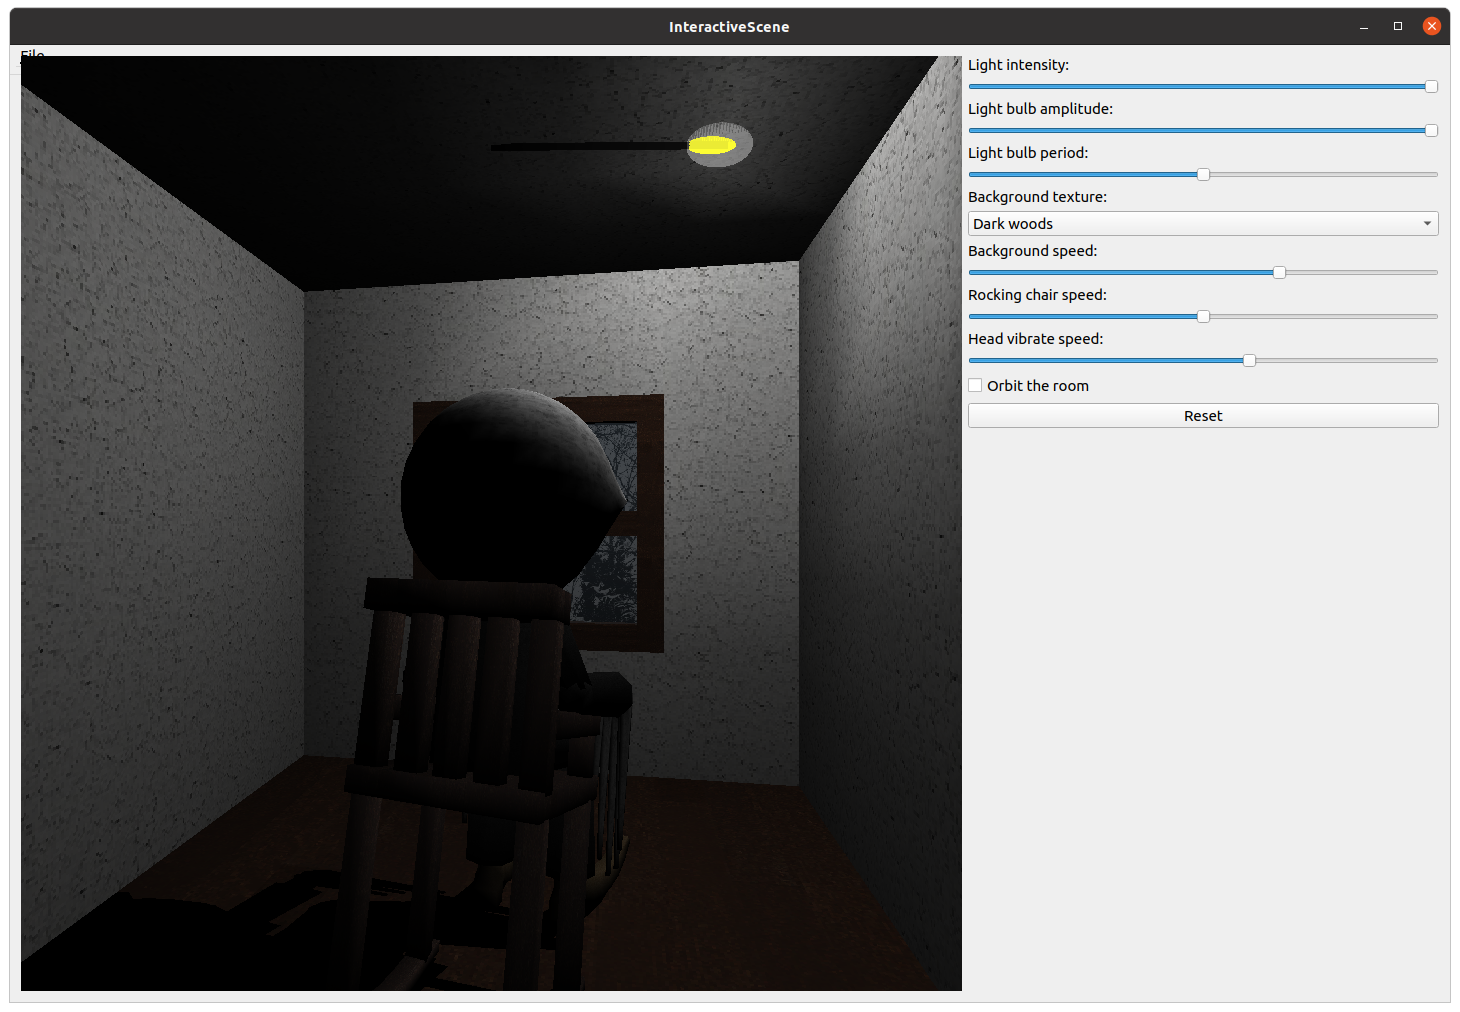
\includegraphics[trim=20 20 500 60, clip, scale=0.2]{shadow-6}
			\caption{Shadows generated from the shadow transform}
			\label{shadow-reel}
		\end{figure}

	\clearpage
	\section{Conclusion}
	Overall I feel that I have been able to meet the technical requirements of the project, having implemented various
	techniques in OpenGL to draw, texture and illuminate objects in a 3D animated scene, as well as the accompanying
	Qt user interface to interact with it. I was also able to learn how to create 3D models from convex shapes and polygons
	using 3DS Max.
	
	\bigskip
	
	The general feedback from users on viewing the scene hint at discomfort, surprise and creepiness. This is in my opinion
	a success in creating a horrific atmosphere set out in the aims of the project, as the scene has been 
	able to illicit similar emotions to the works I have drawn inspiration from.

	\subsection{Source code instructions}
	To run the application from source, enter the following commands from the project directory in a terminal:
	
	\bigskip
	
	\noindent
	\texttt{cd src\\qmake\\make\\./InteractiveScene}
	
	\subsection{Video demonstrations}
	Software was tested using feng-linux/gpu however unfortunately subject to lower frame rates through the service.
	Video demonstrations of the scene running at full-speed are available here:
	\begin{itemize}
		\item \url{https://youtu.be/I-vPSETKljw}
		\item \url{https://youtu.be/YgDw-1BfJhA}
	\end{itemize}
	
	\subsection{Closing scene}
	\begin{figure}[H]
		\centering	
		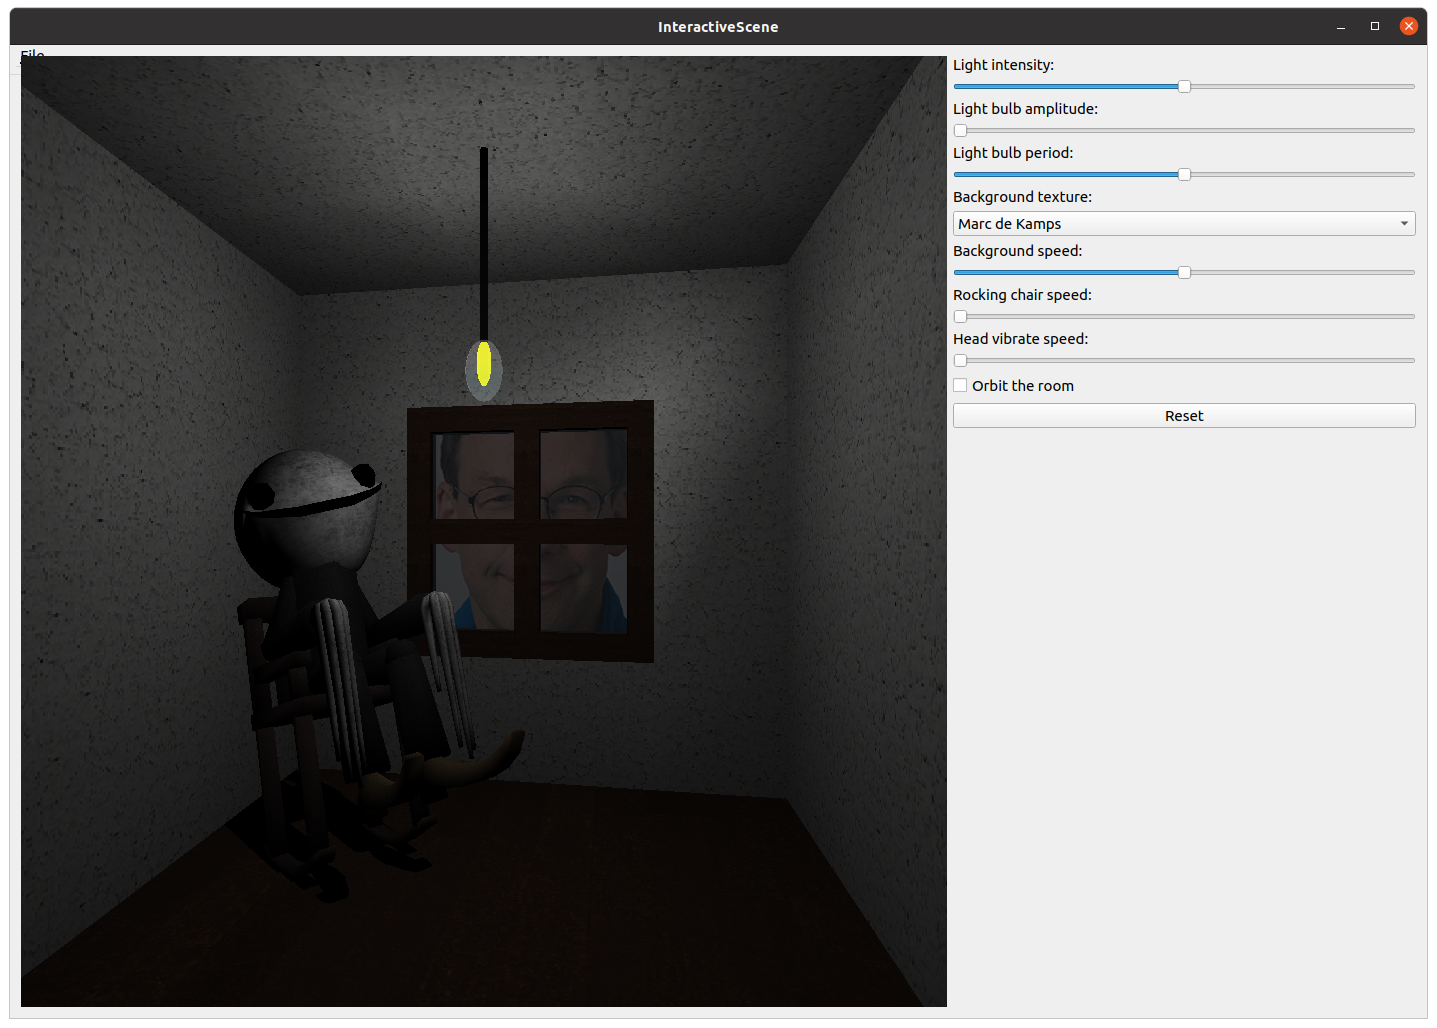
\includegraphics[scale=0.25]{closing-0}
		\caption{Thank you for reading this report!}
		\label{closing-scene}
	\end{figure}
\end{document}